% Options for packages loaded elsewhere
\PassOptionsToPackage{unicode}{hyperref}
\PassOptionsToPackage{hyphens}{url}
\PassOptionsToPackage{dvipsnames,svgnames,x11names}{xcolor}
%
\documentclass[
  ignorenonframetext,
]{beamer}
\title{Mixed Models}
\author{Zack Treisman}
\date{Spring 2022}

\usepackage{pgfpages}
\setbeamertemplate{caption}[numbered]
\setbeamertemplate{caption label separator}{: }
\setbeamercolor{caption name}{fg=normal text.fg}
\beamertemplatenavigationsymbolsempty
% Prevent slide breaks in the middle of a paragraph
\widowpenalties 1 10000
\raggedbottom
\setbeamertemplate{part page}{
  \centering
  \begin{beamercolorbox}[sep=16pt,center]{part title}
    \usebeamerfont{part title}\insertpart\par
  \end{beamercolorbox}
}
\setbeamertemplate{section page}{
  \centering
  \begin{beamercolorbox}[sep=12pt,center]{part title}
    \usebeamerfont{section title}\insertsection\par
  \end{beamercolorbox}
}
\setbeamertemplate{subsection page}{
  \centering
  \begin{beamercolorbox}[sep=8pt,center]{part title}
    \usebeamerfont{subsection title}\insertsubsection\par
  \end{beamercolorbox}
}
\AtBeginPart{
  \frame{\partpage}
}
\AtBeginSection{
  \ifbibliography
  \else
    \frame{\sectionpage}
  \fi
}
\AtBeginSubsection{
  \frame{\subsectionpage}
}
\usepackage{amsmath,amssymb}
\usepackage{lmodern}
\usepackage{iftex}
\ifPDFTeX
  \usepackage[T1]{fontenc}
  \usepackage[utf8]{inputenc}
  \usepackage{textcomp} % provide euro and other symbols
\else % if luatex or xetex
  \usepackage{unicode-math}
  \defaultfontfeatures{Scale=MatchLowercase}
  \defaultfontfeatures[\rmfamily]{Ligatures=TeX,Scale=1}
\fi
% Use upquote if available, for straight quotes in verbatim environments
\IfFileExists{upquote.sty}{\usepackage{upquote}}{}
\IfFileExists{microtype.sty}{% use microtype if available
  \usepackage[]{microtype}
  \UseMicrotypeSet[protrusion]{basicmath} % disable protrusion for tt fonts
}{}
\makeatletter
\@ifundefined{KOMAClassName}{% if non-KOMA class
  \IfFileExists{parskip.sty}{%
    \usepackage{parskip}
  }{% else
    \setlength{\parindent}{0pt}
    \setlength{\parskip}{6pt plus 2pt minus 1pt}}
}{% if KOMA class
  \KOMAoptions{parskip=half}}
\makeatother
\usepackage{xcolor}
\IfFileExists{xurl.sty}{\usepackage{xurl}}{} % add URL line breaks if available
\IfFileExists{bookmark.sty}{\usepackage{bookmark}}{\usepackage{hyperref}}
\hypersetup{
  pdftitle={Mixed Models},
  pdfauthor={Zack Treisman},
  colorlinks=true,
  linkcolor={Maroon},
  filecolor={Maroon},
  citecolor={blue},
  urlcolor={Blue},
  pdfcreator={LaTeX via pandoc}}
\urlstyle{same} % disable monospaced font for URLs
\newif\ifbibliography
\usepackage{color}
\usepackage{fancyvrb}
\newcommand{\VerbBar}{|}
\newcommand{\VERB}{\Verb[commandchars=\\\{\}]}
\DefineVerbatimEnvironment{Highlighting}{Verbatim}{commandchars=\\\{\}}
% Add ',fontsize=\small' for more characters per line
\usepackage{framed}
\definecolor{shadecolor}{RGB}{248,248,248}
\newenvironment{Shaded}{\begin{snugshade}}{\end{snugshade}}
\newcommand{\AlertTok}[1]{\textcolor[rgb]{0.94,0.16,0.16}{#1}}
\newcommand{\AnnotationTok}[1]{\textcolor[rgb]{0.56,0.35,0.01}{\textbf{\textit{#1}}}}
\newcommand{\AttributeTok}[1]{\textcolor[rgb]{0.77,0.63,0.00}{#1}}
\newcommand{\BaseNTok}[1]{\textcolor[rgb]{0.00,0.00,0.81}{#1}}
\newcommand{\BuiltInTok}[1]{#1}
\newcommand{\CharTok}[1]{\textcolor[rgb]{0.31,0.60,0.02}{#1}}
\newcommand{\CommentTok}[1]{\textcolor[rgb]{0.56,0.35,0.01}{\textit{#1}}}
\newcommand{\CommentVarTok}[1]{\textcolor[rgb]{0.56,0.35,0.01}{\textbf{\textit{#1}}}}
\newcommand{\ConstantTok}[1]{\textcolor[rgb]{0.00,0.00,0.00}{#1}}
\newcommand{\ControlFlowTok}[1]{\textcolor[rgb]{0.13,0.29,0.53}{\textbf{#1}}}
\newcommand{\DataTypeTok}[1]{\textcolor[rgb]{0.13,0.29,0.53}{#1}}
\newcommand{\DecValTok}[1]{\textcolor[rgb]{0.00,0.00,0.81}{#1}}
\newcommand{\DocumentationTok}[1]{\textcolor[rgb]{0.56,0.35,0.01}{\textbf{\textit{#1}}}}
\newcommand{\ErrorTok}[1]{\textcolor[rgb]{0.64,0.00,0.00}{\textbf{#1}}}
\newcommand{\ExtensionTok}[1]{#1}
\newcommand{\FloatTok}[1]{\textcolor[rgb]{0.00,0.00,0.81}{#1}}
\newcommand{\FunctionTok}[1]{\textcolor[rgb]{0.00,0.00,0.00}{#1}}
\newcommand{\ImportTok}[1]{#1}
\newcommand{\InformationTok}[1]{\textcolor[rgb]{0.56,0.35,0.01}{\textbf{\textit{#1}}}}
\newcommand{\KeywordTok}[1]{\textcolor[rgb]{0.13,0.29,0.53}{\textbf{#1}}}
\newcommand{\NormalTok}[1]{#1}
\newcommand{\OperatorTok}[1]{\textcolor[rgb]{0.81,0.36,0.00}{\textbf{#1}}}
\newcommand{\OtherTok}[1]{\textcolor[rgb]{0.56,0.35,0.01}{#1}}
\newcommand{\PreprocessorTok}[1]{\textcolor[rgb]{0.56,0.35,0.01}{\textit{#1}}}
\newcommand{\RegionMarkerTok}[1]{#1}
\newcommand{\SpecialCharTok}[1]{\textcolor[rgb]{0.00,0.00,0.00}{#1}}
\newcommand{\SpecialStringTok}[1]{\textcolor[rgb]{0.31,0.60,0.02}{#1}}
\newcommand{\StringTok}[1]{\textcolor[rgb]{0.31,0.60,0.02}{#1}}
\newcommand{\VariableTok}[1]{\textcolor[rgb]{0.00,0.00,0.00}{#1}}
\newcommand{\VerbatimStringTok}[1]{\textcolor[rgb]{0.31,0.60,0.02}{#1}}
\newcommand{\WarningTok}[1]{\textcolor[rgb]{0.56,0.35,0.01}{\textbf{\textit{#1}}}}
\usepackage{graphicx}
\makeatletter
\def\maxwidth{\ifdim\Gin@nat@width>\linewidth\linewidth\else\Gin@nat@width\fi}
\def\maxheight{\ifdim\Gin@nat@height>\textheight\textheight\else\Gin@nat@height\fi}
\makeatother
% Scale images if necessary, so that they will not overflow the page
% margins by default, and it is still possible to overwrite the defaults
% using explicit options in \includegraphics[width, height, ...]{}
\setkeys{Gin}{width=\maxwidth,height=\maxheight,keepaspectratio}
% Set default figure placement to htbp
\makeatletter
\def\fps@figure{htbp}
\makeatother
\setlength{\emergencystretch}{3em} % prevent overfull lines
\providecommand{\tightlist}{%
  \setlength{\itemsep}{0pt}\setlength{\parskip}{0pt}}
\setcounter{secnumdepth}{-\maxdimen} % remove section numbering
\newlength{\cslhangindent}
\setlength{\cslhangindent}{1.5em}
\newlength{\csllabelwidth}
\setlength{\csllabelwidth}{3em}
\newlength{\cslentryspacingunit} % times entry-spacing
\setlength{\cslentryspacingunit}{\parskip}
\newenvironment{CSLReferences}[2] % #1 hanging-ident, #2 entry spacing
 {% don't indent paragraphs
  \setlength{\parindent}{0pt}
  % turn on hanging indent if param 1 is 1
  \ifodd #1
  \let\oldpar\par
  \def\par{\hangindent=\cslhangindent\oldpar}
  \fi
  % set entry spacing
  \setlength{\parskip}{#2\cslentryspacingunit}
 }%
 {}
\usepackage{calc}
\newcommand{\CSLBlock}[1]{#1\hfill\break}
\newcommand{\CSLLeftMargin}[1]{\parbox[t]{\csllabelwidth}{#1}}
\newcommand{\CSLRightInline}[1]{\parbox[t]{\linewidth - \csllabelwidth}{#1}\break}
\newcommand{\CSLIndent}[1]{\hspace{\cslhangindent}#1}

\pgfdeclareimage[width=3.5cm]{mcslogo}{../images/western_logo_hor_MCS_3C_pos.pdf}
\pgfdeclareimage[width=1cm]{ccbysa}{../images/ccbysa88x31.png}
\titlegraphic{\href{http://creativecommons.org/licenses/by-sa/4.0/}{\pgfuseimage{ccbysa}}
\hfill
\href{https://western.edu/program/mathematics/}{\pgfuseimage{mcslogo}}}
%\usecolortheme{wcu}
%\institute{Western Colorado University}
%\setbeamertemplate{navigation symbols}{}
\ifLuaTeX
  \usepackage{selnolig}  % disable illegal ligatures
\fi

\begin{document}
\frame{\titlepage}

\begin{frame}[fragile]
\begin{Shaded}
\begin{Highlighting}[]
\FunctionTok{library}\NormalTok{(dplyr)}
\FunctionTok{library}\NormalTok{(ggplot2)}
\FunctionTok{library}\NormalTok{(nlme)}
\FunctionTok{library}\NormalTok{(MuMIn)}
\FunctionTok{library}\NormalTok{(car)}
\FunctionTok{library}\NormalTok{(glmmTMB)}
\FunctionTok{library}\NormalTok{(mgcv)}
\FunctionTok{library}\NormalTok{(MASS)}
\FunctionTok{library}\NormalTok{(brms)}
\FunctionTok{set.seed}\NormalTok{(}\DecValTok{3}\NormalTok{)}
\end{Highlighting}
\end{Shaded}
\end{frame}

\begin{frame}{Philosophy}
\protect\hypertarget{philosophy}{}
The tools we will investigate this week address several related issues.

\begin{itemize}
\tightlist
\item
  Heterogeneity of variance

  \begin{itemize}
  \tightlist
  \item
    Sometimes this is definitely present, even after building an
    otherwise good model.
  \end{itemize}
\item
  Nuisance variables

  \begin{itemize}
  \tightlist
  \item
    Often, we have variables that we know we need to measure and account
    for, but they are not of primary interest.
  \end{itemize}
\item
  Dependent observations

  \begin{itemize}
  \tightlist
  \item
    The independence assumption implicit in all of our models thus far
    is often false.
  \end{itemize}
\end{itemize}

We do have tools that deal with these issues. If your data are
especially nice and your analysis is fairly straightforward, so are the
tools for building appropriate models. If you are not so lucky, then
things get complicated.
\end{frame}

\begin{frame}{Heterogeneity of variance}
\protect\hypertarget{heterogeneity-of-variance}{}
Why is the variance heterogenous?

\begin{itemize}
\tightlist
\item
  Because of a variable. Hopefully one in your data.
\end{itemize}

It's possible that the heterogeneity is from not looking at the
variables in your model at appropriate scales.

\begin{itemize}
\tightlist
\item
  Were the data collected on the same scale that you are using, or have
  you transformed any variables? Recall that inverting a log-transform
  changes additive error into multiplicative error. Any nonlinear
  variable transform does this.
\end{itemize}
\end{frame}

\begin{frame}{Nuisance variables}
\protect\hypertarget{nuisance-variables}{}
There is no set definition of nuisance variable. These are any variables
that you know are having an effect on your response but are not what you
are trying to investigate.

\begin{itemize}
\tightlist
\item
  Be sure you think about why you aren't interested.
\end{itemize}

Accounting for these variables is essential for establishing appropriate
baselines. Sometimes the signal that you are trying to measure is small
compared to environmental variation.

\begin{itemize}
\tightlist
\item
  Effect of compost treatment on soil moisture retention is going to be
  smaller than rainfall, soil characteristics, etc. (Cooper)
\end{itemize}
\end{frame}

\begin{frame}{Dependent observations}
\protect\hypertarget{dependent-observations}{}
Measurements on the same or similar individuals are not independent.

\begin{itemize}
\tightlist
\item
  Individual what? (organism, forest, drainage, \ldots)
\end{itemize}

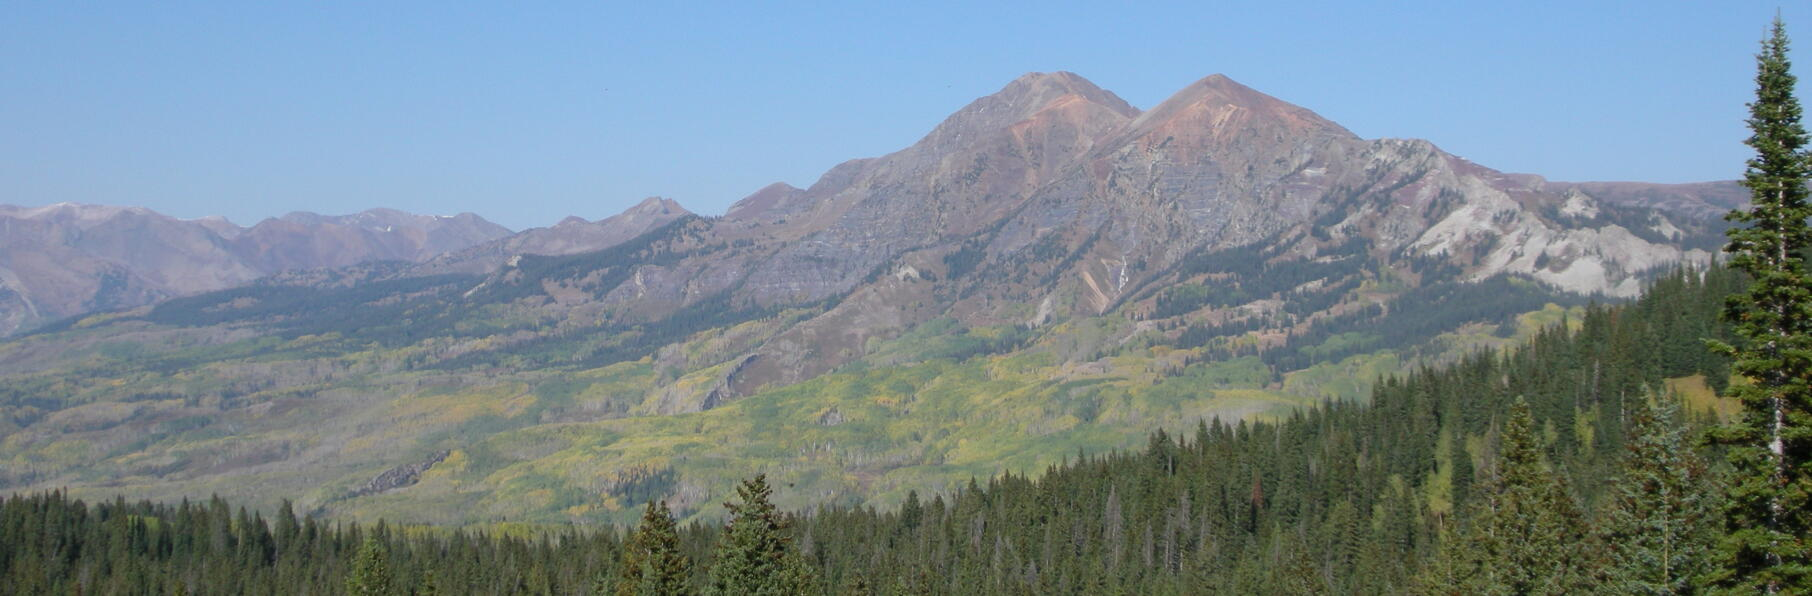
\includegraphics[width=\textwidth,height=0.4\textheight]{../images/ruby.jpg}

Having dependent observations means that your data set is effectively
smaller.

\begin{itemize}
\tightlist
\item
  Sample from enough individuals so that you get a statistically
  meaningful set of observations. (sufficient power)
\end{itemize}
\end{frame}

\begin{frame}[fragile]{Tools}
\protect\hypertarget{tools}{}
\begin{itemize}
\tightlist
\item
  \textbf{Mixed effects models} (LMM, GLMM, GAMM)

  \begin{itemize}
  \tightlist
  \item
    Fixed effect variables modify the signal, random effect variables
    modify the noise.
  \item
    Many packages for this, no clear winner. (\texttt{lme4} has
    \texttt{lmer}, \texttt{glmer} and \texttt{nlmer}; \texttt{nlme} has
    \texttt{lme}; \texttt{MASS} has \texttt{glmmPQL}; \texttt{glmmTMB}
    has \texttt{glmmTMB}. Bayesian options include \texttt{brms::brm}
    and \texttt{MCMCglmm::MCMCglmm}.)
  \item
    Hopefully this will be easier in another decade or so.
  \end{itemize}
\item
  Also see \textbf{Generalized least squares} (GLS) and
  \textbf{Generalized estimating equations} (GEE).
\end{itemize}

Many of the tools for mixed modeling also allow the specification of
structure to correlation (\texttt{corStruct}) and variance
(\texttt{varStruct}).
\end{frame}

\begin{frame}{Owls}
\protect\hypertarget{owls}{}
Roulin and Bersier (2007) (a running example in Zuur et al. (2009))
investigates begging behavior in nestling barn owls.
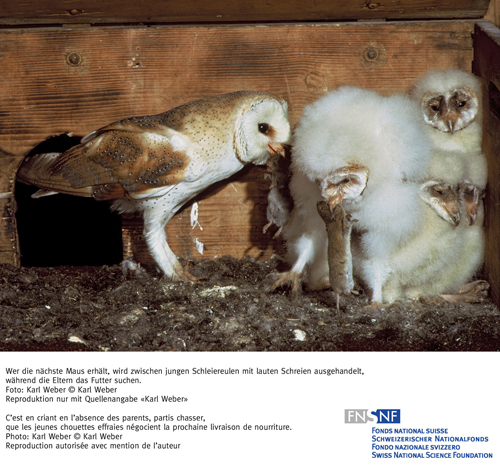
\includegraphics[width=\textwidth,height=0.7\textheight]{../images/owls.jpg}
They ask if vocal intensity of owl chick begging differs by parent.
\end{frame}

\begin{frame}[fragile]{Owl data}
\protect\hypertarget{owl-data}{}
The data are in the package \texttt{glmmTMB}.

\tiny

\begin{Shaded}
\begin{Highlighting}[]
\FunctionTok{head}\NormalTok{(Owls,}\DecValTok{3}\NormalTok{)}
\end{Highlighting}
\end{Shaded}

\begin{verbatim}
##         Nest FoodTreatment SexParent ArrivalTime SiblingNegotiation BroodSize
## 1 AutavauxTV      Deprived      Male       22.25                  4         5
## 2 AutavauxTV      Satiated      Male       22.38                  0         5
## 3 AutavauxTV      Deprived      Male       22.53                  2         5
##   NegPerChick logBroodSize
## 1         0.8     1.609438
## 2         0.0     1.609438
## 3         0.4     1.609438
\end{verbatim}

\normalsize

Without other predictors, it does not appear that begging frequency
depends on the parent.
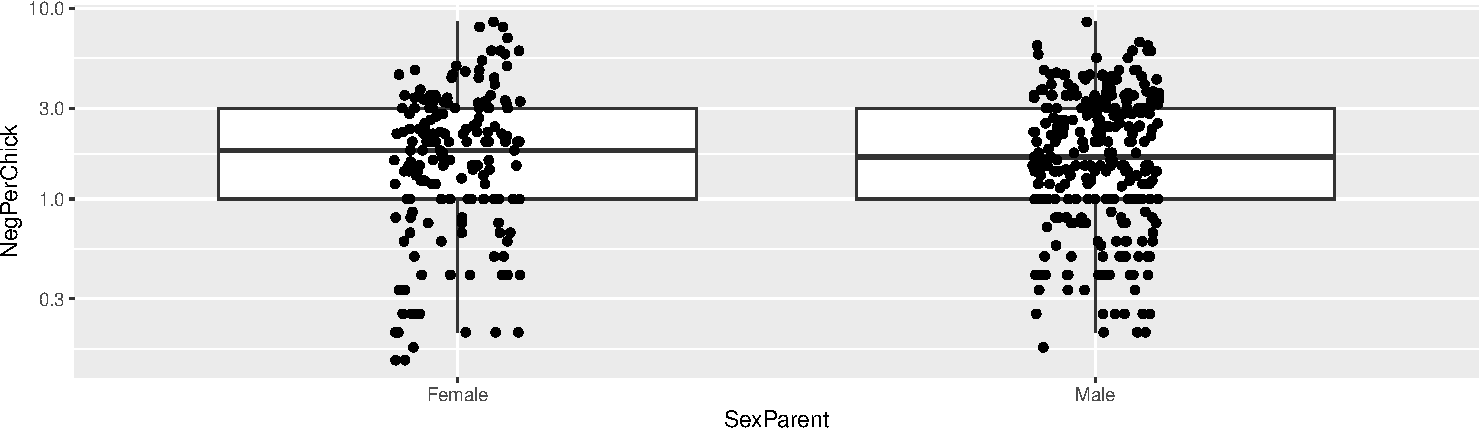
\includegraphics{mixed_models_files/figure-beamer/unnamed-chunk-4-1.pdf}
\end{frame}

\begin{frame}{Food Treatment}
\protect\hypertarget{food-treatment}{}
Begging behavior is likely affected by the hunger levels in the nest.
The researchers imposed this as an experimental treatment to control for
unknown variation. Feed some nests extra, deprive others, then swap
treatments the following night.

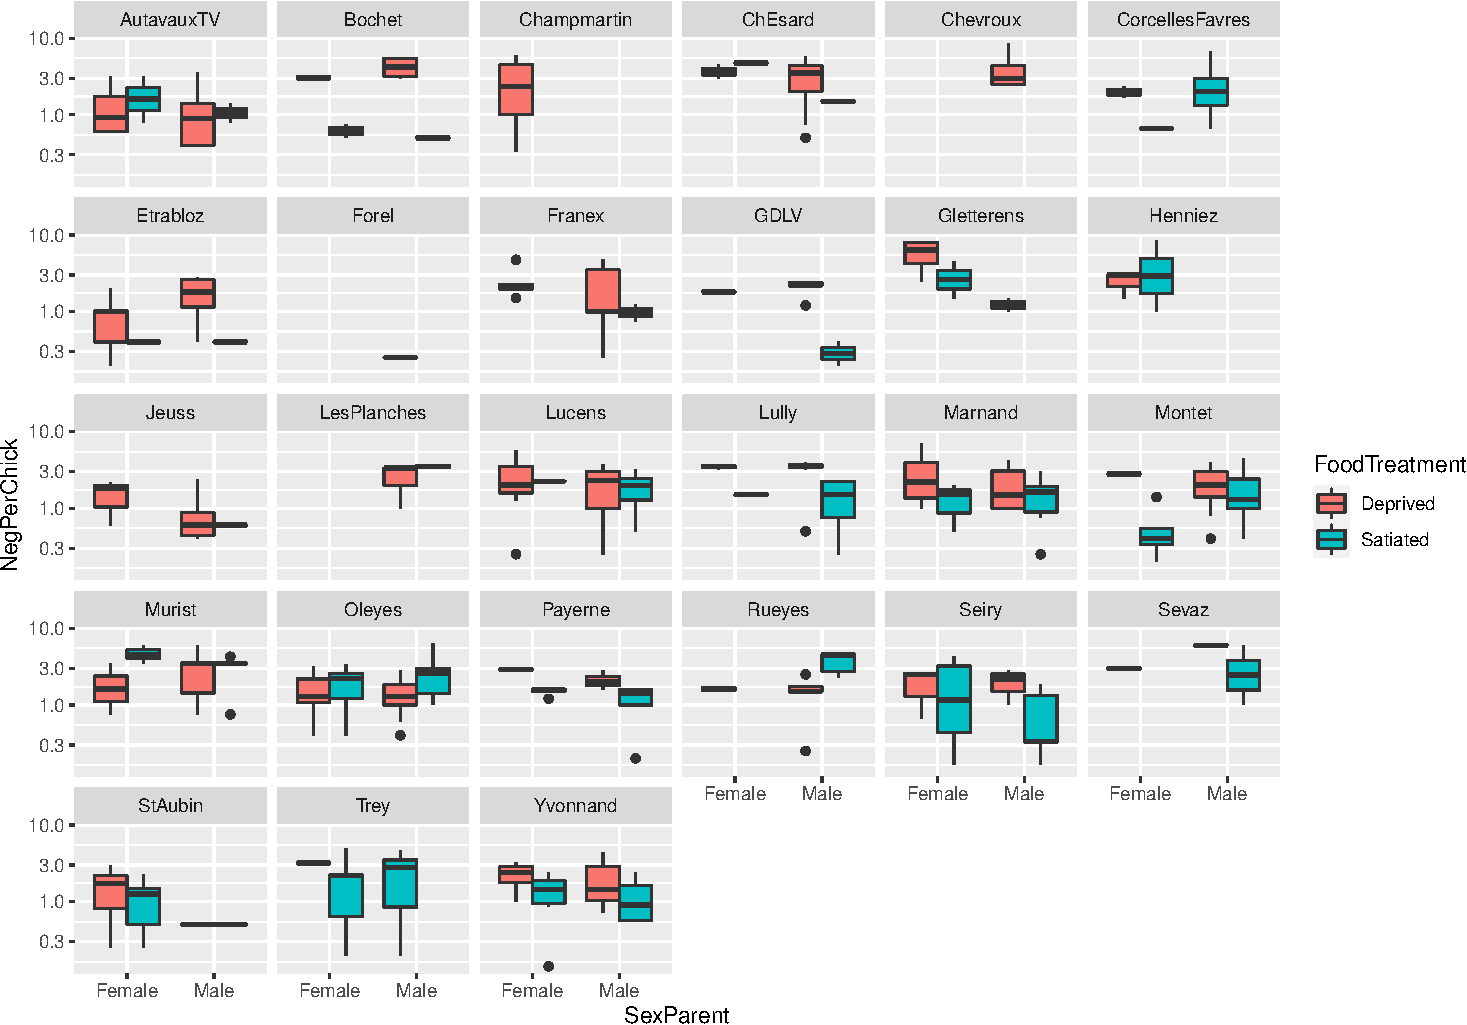
\includegraphics{mixed_models_files/figure-beamer/unnamed-chunk-5-1.pdf}

Still no visible difference between parents.
\end{frame}

\begin{frame}{Nest is a nuisance varaible.}
\protect\hypertarget{nest-is-a-nuisance-varaible.}{}
\scriptsize

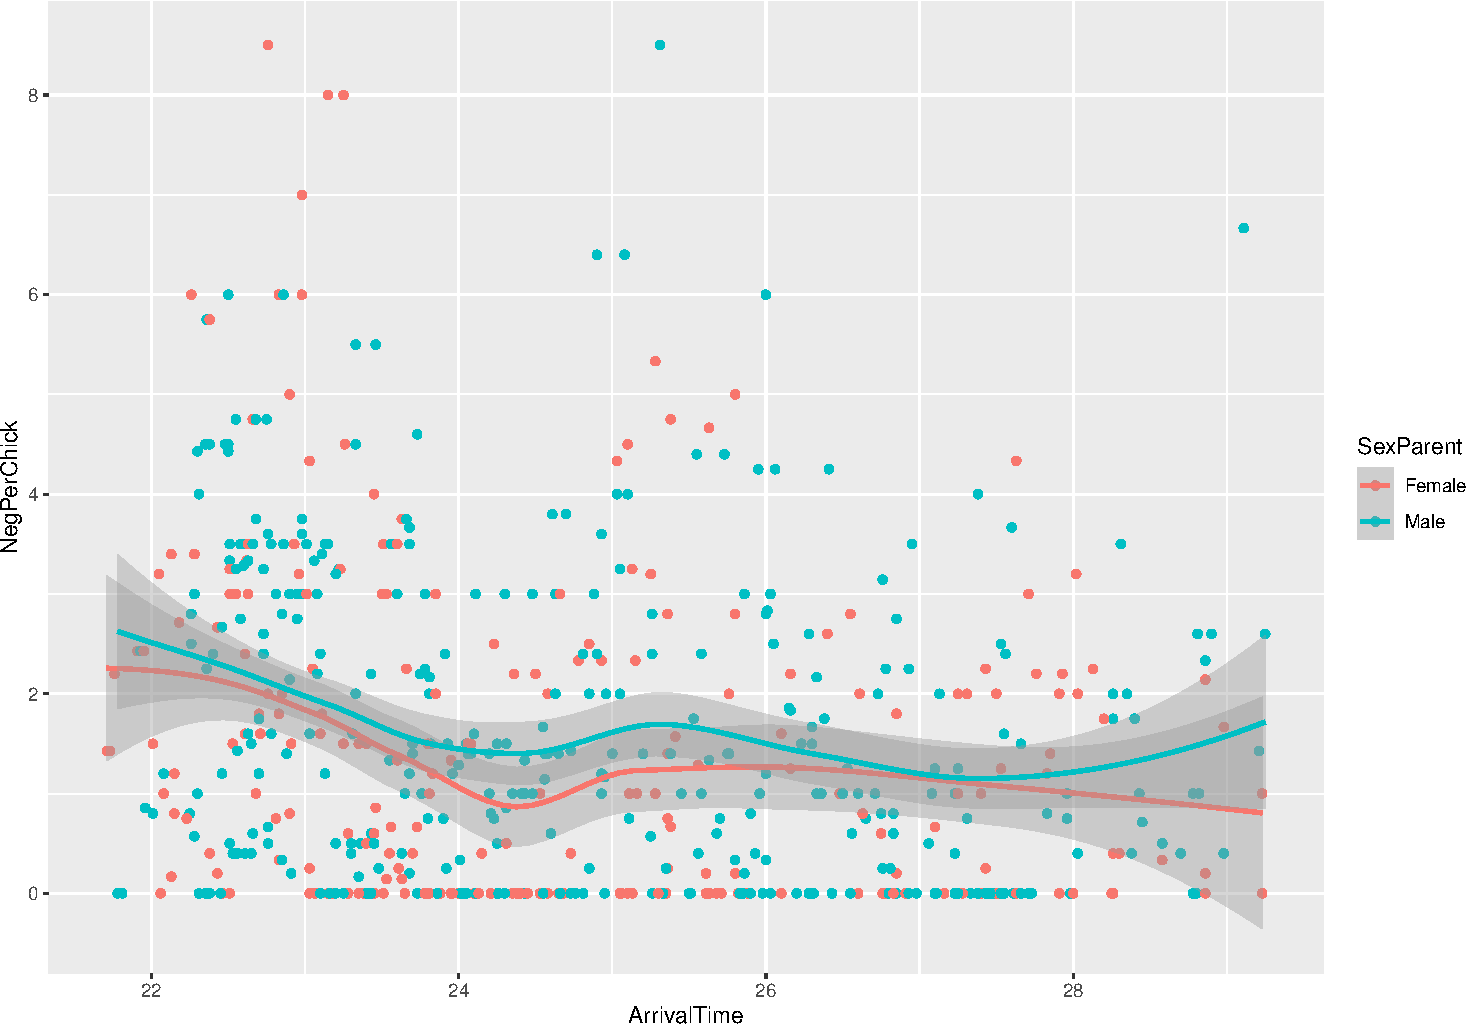
\includegraphics{mixed_models_files/figure-beamer/unnamed-chunk-6-1.pdf}
\end{frame}

\begin{frame}{Arrival time affects the variance.}
\protect\hypertarget{arrival-time-affects-the-variance.}{}
It could also be correlated with the sex of the parent.

\scriptsize

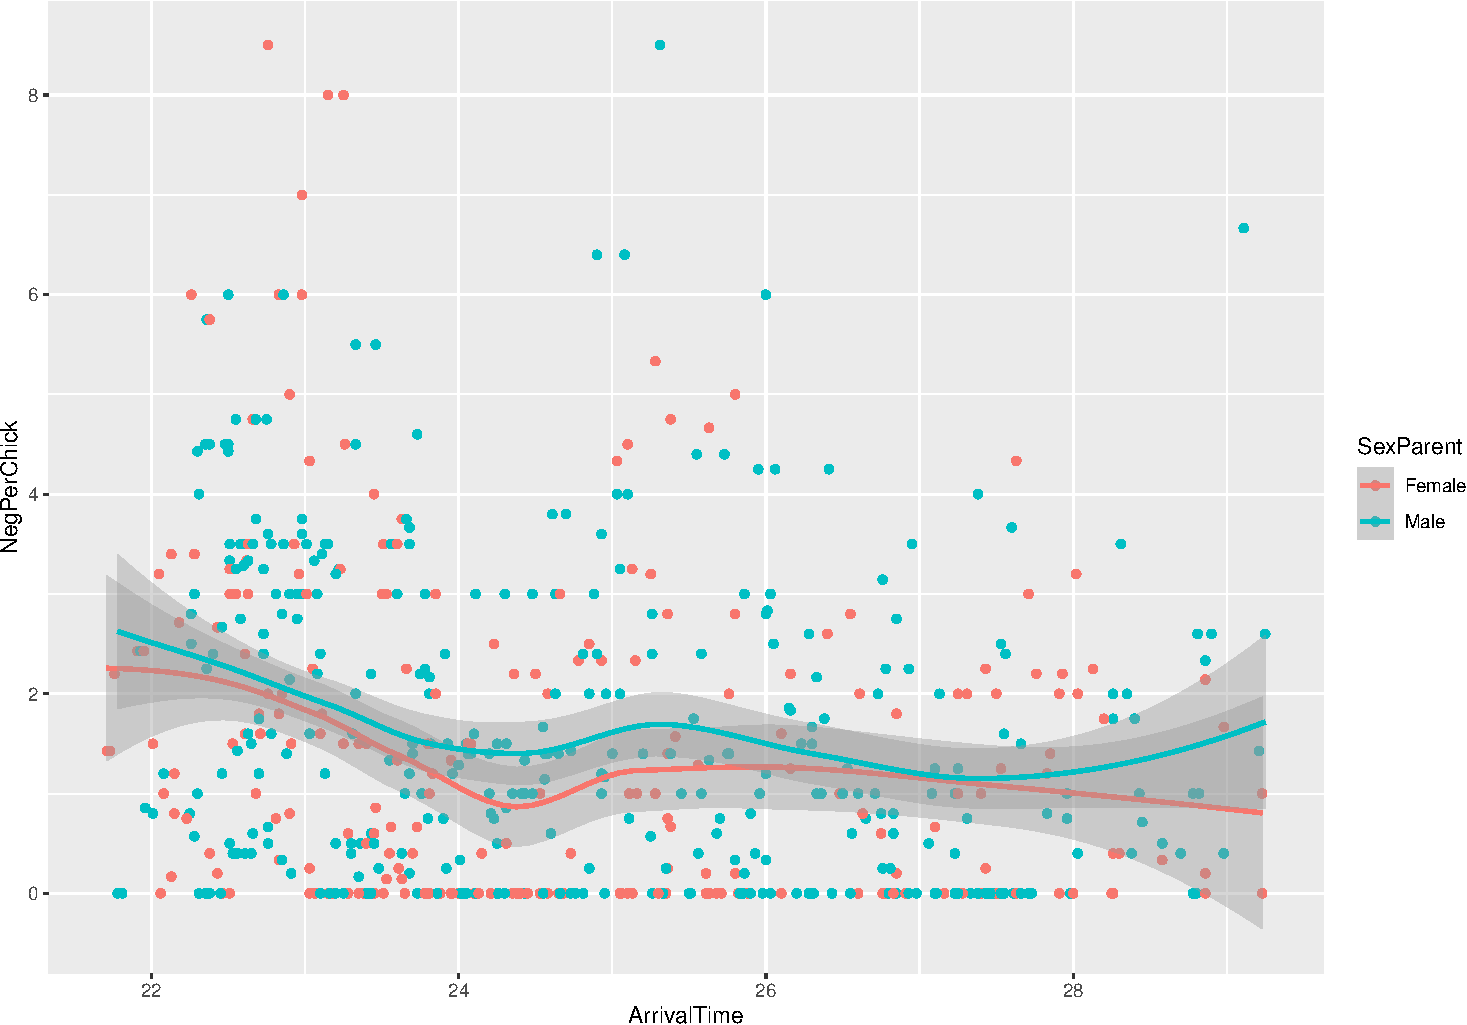
\includegraphics{mixed_models_files/figure-beamer/unnamed-chunk-7-1.pdf}
\end{frame}

\begin{frame}[fragile]{Linear model}
\protect\hypertarget{linear-model}{}
First thing to try is basic linear regression (ANCOVA).

\scriptsize

\begin{Shaded}
\begin{Highlighting}[]
\NormalTok{M.lm }\OtherTok{\textless{}{-}} \FunctionTok{lm}\NormalTok{(NegPerChick}\SpecialCharTok{\textasciitilde{}}\NormalTok{SexParent}\SpecialCharTok{*}\NormalTok{(FoodTreatment}\SpecialCharTok{+}\NormalTok{ArrivalTime),}\AttributeTok{data=}\NormalTok{Owls)}
\end{Highlighting}
\end{Shaded}

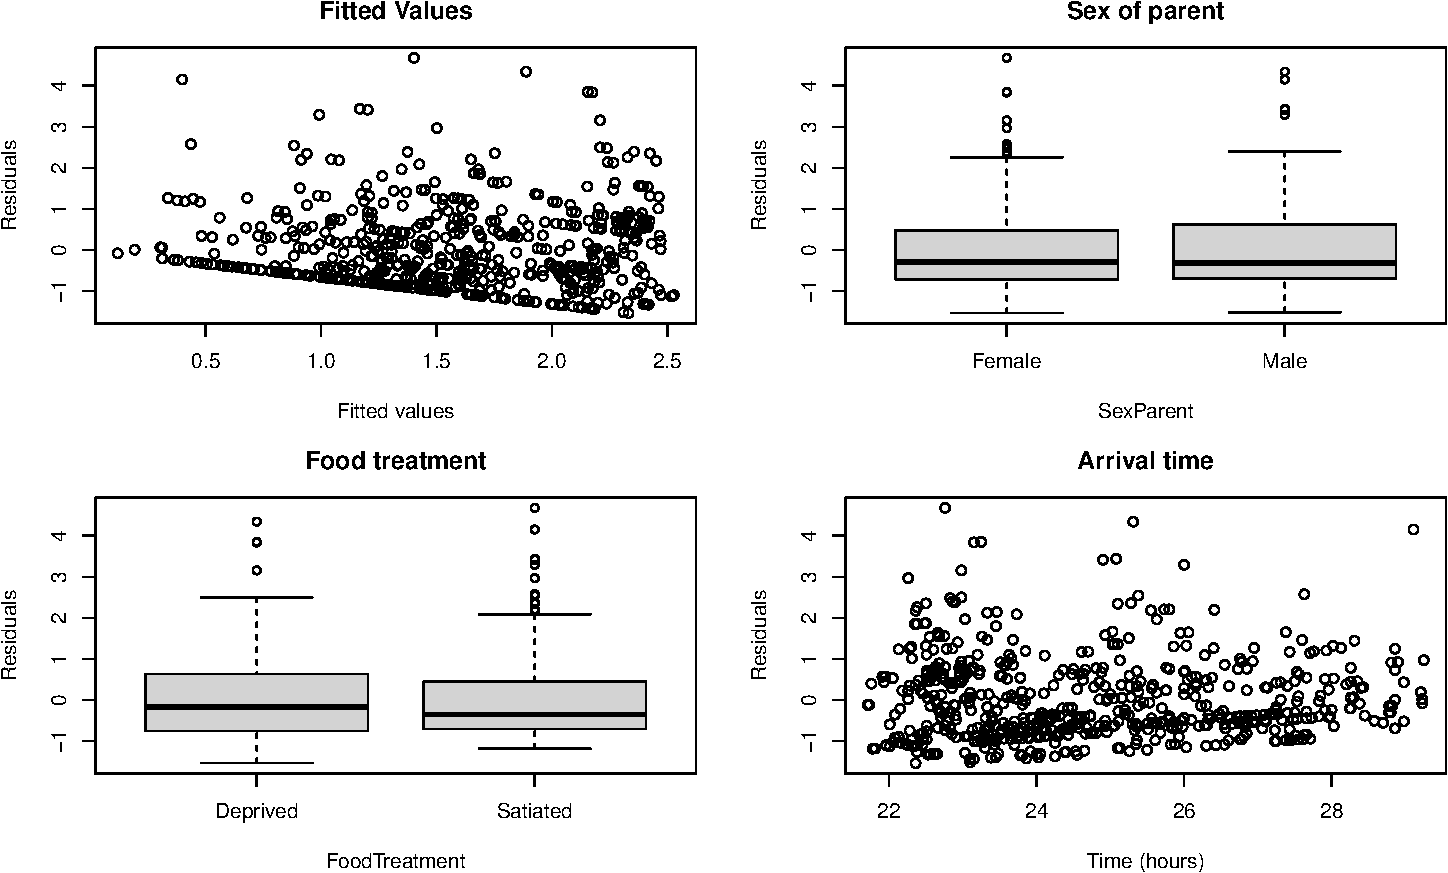
\includegraphics{mixed_models_files/figure-beamer/unnamed-chunk-9-1.pdf}
\end{frame}

\begin{frame}[fragile]{Code for those diagnostic plots}
\protect\hypertarget{code-for-those-diagnostic-plots}{}
From Zuur et al. (2009).

\scriptsize

\begin{Shaded}
\begin{Highlighting}[]
\NormalTok{Elm}\OtherTok{=}\FunctionTok{rstandard}\NormalTok{(M.lm);  Flm}\OtherTok{\textless{}{-}}\FunctionTok{fitted}\NormalTok{(M.lm)}
\NormalTok{op}\OtherTok{\textless{}{-}}\FunctionTok{par}\NormalTok{(}\AttributeTok{mfrow=}\FunctionTok{c}\NormalTok{(}\DecValTok{2}\NormalTok{,}\DecValTok{2}\NormalTok{),}\AttributeTok{mar=}\FunctionTok{c}\NormalTok{(}\DecValTok{4}\NormalTok{,}\DecValTok{4}\NormalTok{,}\DecValTok{3}\NormalTok{,}\DecValTok{2}\NormalTok{)) }
\NormalTok{MyYlab}\OtherTok{=}\StringTok{"Residuals"}
\FunctionTok{plot}\NormalTok{(}\AttributeTok{x=}\NormalTok{Flm,}\AttributeTok{y=}\NormalTok{Elm, }
     \AttributeTok{xlab=}\StringTok{"Fitted values"}\NormalTok{,}\AttributeTok{ylab=}\NormalTok{MyYlab, }\AttributeTok{main =} \StringTok{"Fitted Values"}\NormalTok{)}
\FunctionTok{boxplot}\NormalTok{(Elm}\SpecialCharTok{\textasciitilde{}}\NormalTok{SexParent,}\AttributeTok{data=}\NormalTok{Owls,}
        \AttributeTok{main=}\StringTok{"Sex of parent"}\NormalTok{,}\AttributeTok{ylab=}\NormalTok{MyYlab)}
\FunctionTok{boxplot}\NormalTok{(Elm}\SpecialCharTok{\textasciitilde{}}\NormalTok{FoodTreatment,}\AttributeTok{data=}\NormalTok{Owls,}
        \AttributeTok{main=}\StringTok{"Food treatment"}\NormalTok{,}\AttributeTok{ylab=}\NormalTok{MyYlab)}
\FunctionTok{plot}\NormalTok{(}\AttributeTok{x=}\NormalTok{Owls}\SpecialCharTok{$}\NormalTok{ArrivalTime,}\AttributeTok{y=}\NormalTok{Elm,}
     \AttributeTok{main=}\StringTok{"Arrival time"}\NormalTok{,}\AttributeTok{ylab=}\NormalTok{MyYlab,}\AttributeTok{xlab=}\StringTok{"Time (hours)"}\NormalTok{)}
\FunctionTok{par}\NormalTok{(op)}
\end{Highlighting}
\end{Shaded}
\end{frame}

\begin{frame}[fragile]{Summary of \texttt{M.lm}}
\protect\hypertarget{summary-of-m.lm}{}
\tiny

\begin{verbatim}
## 
## Call:
## lm(formula = NegPerChick ~ SexParent * (FoodTreatment + ArrivalTime), 
##     data = Owls)
## 
## Residuals:
##     Min      1Q  Median      3Q     Max 
## -2.3317 -1.0833 -0.4573  0.8630  7.0978 
## 
## Coefficients:
##                                      Estimate Std. Error t value Pr(>|t|)    
## (Intercept)                          6.766988   1.259815   5.371 1.12e-07 ***
## SexParentMale                       -0.044492   1.652324  -0.027    0.979    
## FoodTreatmentSatiated               -0.850112   0.195174  -4.356 1.56e-05 ***
## ArrivalTime                         -0.198358   0.050578  -3.922 9.81e-05 ***
## SexParentMale:FoodTreatmentSatiated  0.086027   0.254579   0.338    0.736    
## SexParentMale:ArrivalTime            0.007349   0.066230   0.111    0.912    
## ---
## Signif. codes:  0 '***' 0.001 '**' 0.01 '*' 0.05 '.' 0.1 ' ' 1
## 
## Residual standard error: 1.527 on 593 degrees of freedom
## Multiple R-squared:  0.1134, Adjusted R-squared:  0.1059 
## F-statistic: 15.16 on 5 and 593 DF,  p-value: 4.941e-14
\end{verbatim}

\normalsize

Note the low \(R^2\).
\end{frame}

\begin{frame}[fragile]{Log-transform the negotiations per chick}
\protect\hypertarget{log-transform-the-negotiations-per-chick}{}
This helps some with the non-normality and heteroscedasticity in
variance.

\scriptsize

\begin{Shaded}
\begin{Highlighting}[]
\NormalTok{Owls}\SpecialCharTok{$}\NormalTok{LogNeg}\OtherTok{\textless{}{-}}\FunctionTok{log}\NormalTok{(Owls}\SpecialCharTok{$}\NormalTok{NegPerChick}\SpecialCharTok{+}\DecValTok{1}\NormalTok{)}
\NormalTok{M2.lm}\OtherTok{=}\FunctionTok{lm}\NormalTok{(LogNeg}\SpecialCharTok{\textasciitilde{}}\NormalTok{SexParent}\SpecialCharTok{*}\NormalTok{(FoodTreatment}\SpecialCharTok{+}\NormalTok{ArrivalTime),}\AttributeTok{data=}\NormalTok{Owls)}
\end{Highlighting}
\end{Shaded}

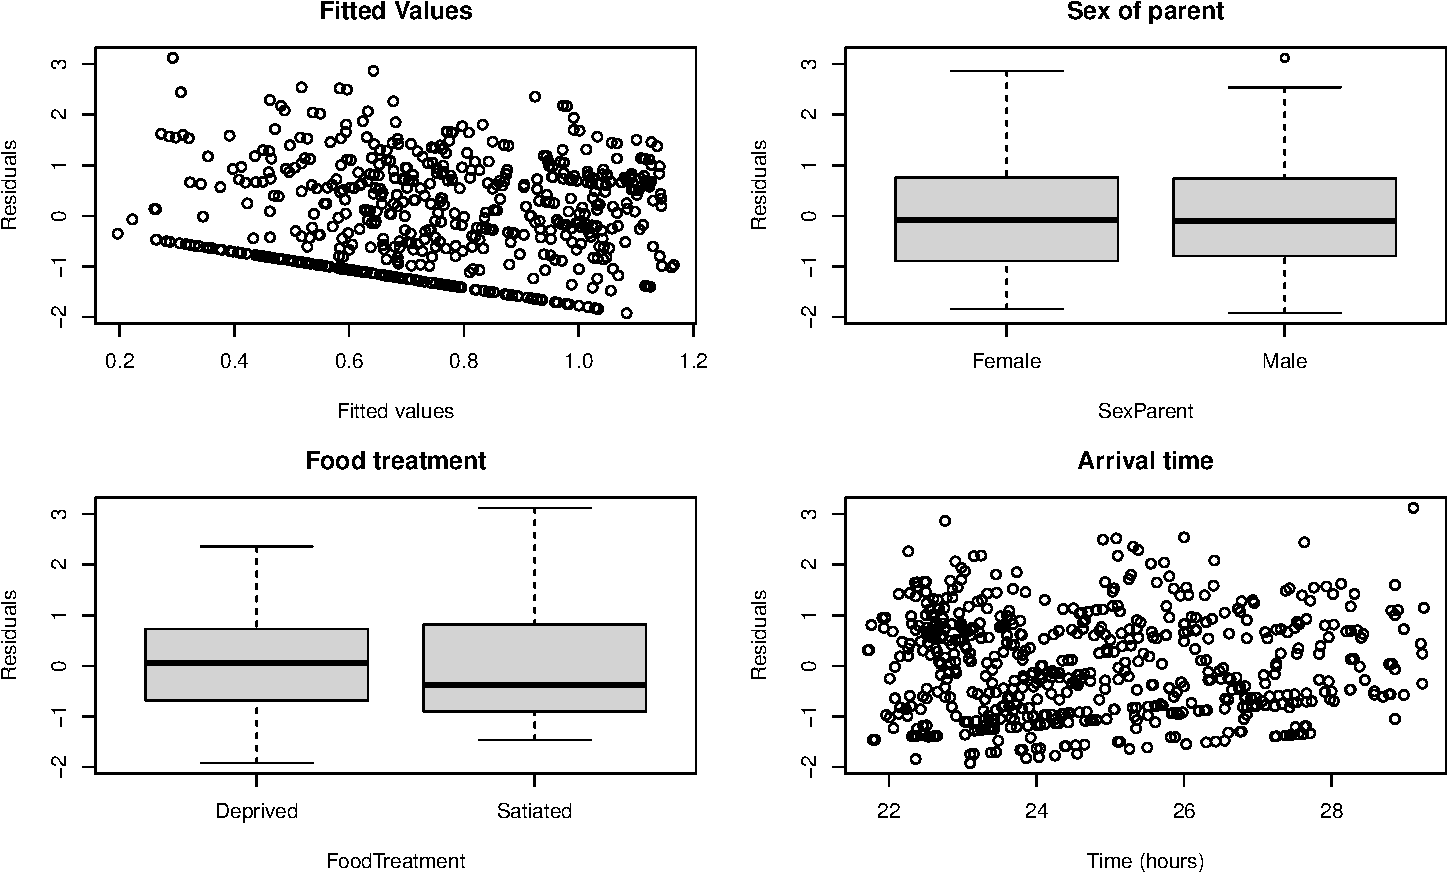
\includegraphics{mixed_models_files/figure-beamer/unnamed-chunk-13-1.pdf}
\end{frame}

\begin{frame}[fragile]{Summary of \texttt{M2.lm}}
\protect\hypertarget{summary-of-m2.lm}{}
\tiny

\begin{verbatim}
## 
## Call:
## lm(formula = LogNeg ~ SexParent * (FoodTreatment + ArrivalTime), 
##     data = Owls)
## 
## Residuals:
##      Min       1Q   Median       3Q      Max 
## -1.08353 -0.46500 -0.05645  0.41842  1.74442 
## 
## Coefficients:
##                                      Estimate Std. Error t value Pr(>|t|)    
## (Intercept)                          2.574961   0.466240   5.523 5.00e-08 ***
## SexParentMale                        0.176201   0.611502   0.288 0.773336    
## FoodTreatmentSatiated               -0.364079   0.072231  -5.040 6.18e-07 ***
## ArrivalTime                         -0.068917   0.018718  -3.682 0.000253 ***
## SexParentMale:FoodTreatmentSatiated  0.006885   0.094216   0.073 0.941767    
## SexParentMale:ArrivalTime           -0.003275   0.024511  -0.134 0.893745    
## ---
## Signif. codes:  0 '***' 0.001 '**' 0.01 '*' 0.05 '.' 0.1 ' ' 1
## 
## Residual standard error: 0.5649 on 593 degrees of freedom
## Multiple R-squared:  0.1402, Adjusted R-squared:  0.133 
## F-statistic: 19.35 on 5 and 593 DF,  p-value: < 2.2e-16
\end{verbatim}

\normalsize

Still a low \(R^2\). We are missing most of the signal.
\end{frame}

\begin{frame}[fragile]{A mixed model with \texttt{nlme::lme}}
\protect\hypertarget{a-mixed-model-with-nlmelme}{}
Refit the linear model with \texttt{nlme::gls} so that it can be more
easily compared to the mixed model. The fitted model is identical to the
one above, but R puts it in a different namespace.

\begin{itemize}
\tightlist
\item
  The argument \texttt{random=\textasciitilde{}1\textbar{}Nest} in
  \texttt{lme} indicates that the intercept varies depending on the
  nest.
\item
  Since observations from the same nest are correlated, the effective
  number of observations is reduced.
\item
  The \texttt{anova} command carries out a likelihood ratio test since
  we give it \texttt{lme} objects.
\end{itemize}

\scriptsize

\begin{Shaded}
\begin{Highlighting}[]
\NormalTok{Form }\OtherTok{\textless{}{-}} \FunctionTok{formula}\NormalTok{(LogNeg}\SpecialCharTok{\textasciitilde{}}\NormalTok{SexParent}\SpecialCharTok{*}\NormalTok{(FoodTreatment}\SpecialCharTok{+}\NormalTok{ArrivalTime))}
\NormalTok{M.gls }\OtherTok{\textless{}{-}} \FunctionTok{gls}\NormalTok{(Form,}\AttributeTok{data=}\NormalTok{Owls)}
\NormalTok{M1.lme }\OtherTok{\textless{}{-}} \FunctionTok{lme}\NormalTok{(Form,}\AttributeTok{random=}\SpecialCharTok{\textasciitilde{}}\DecValTok{1}\SpecialCharTok{|}\NormalTok{Nest,}\AttributeTok{data=}\NormalTok{Owls)}
\FunctionTok{anova}\NormalTok{(M.gls,M1.lme)}
\end{Highlighting}
\end{Shaded}

\begin{verbatim}
##        Model df      AIC      BIC    logLik   Test  L.Ratio p-value
## M.gls      1  7 1053.537 1084.233 -519.7683                        
## M1.lme     2  8 1026.878 1061.959 -505.4390 1 vs 2 28.65875  <.0001
\end{verbatim}
\end{frame}

\begin{frame}{Diagnostic plots of the mixed model}
\protect\hypertarget{diagnostic-plots-of-the-mixed-model}{}
\scriptsize

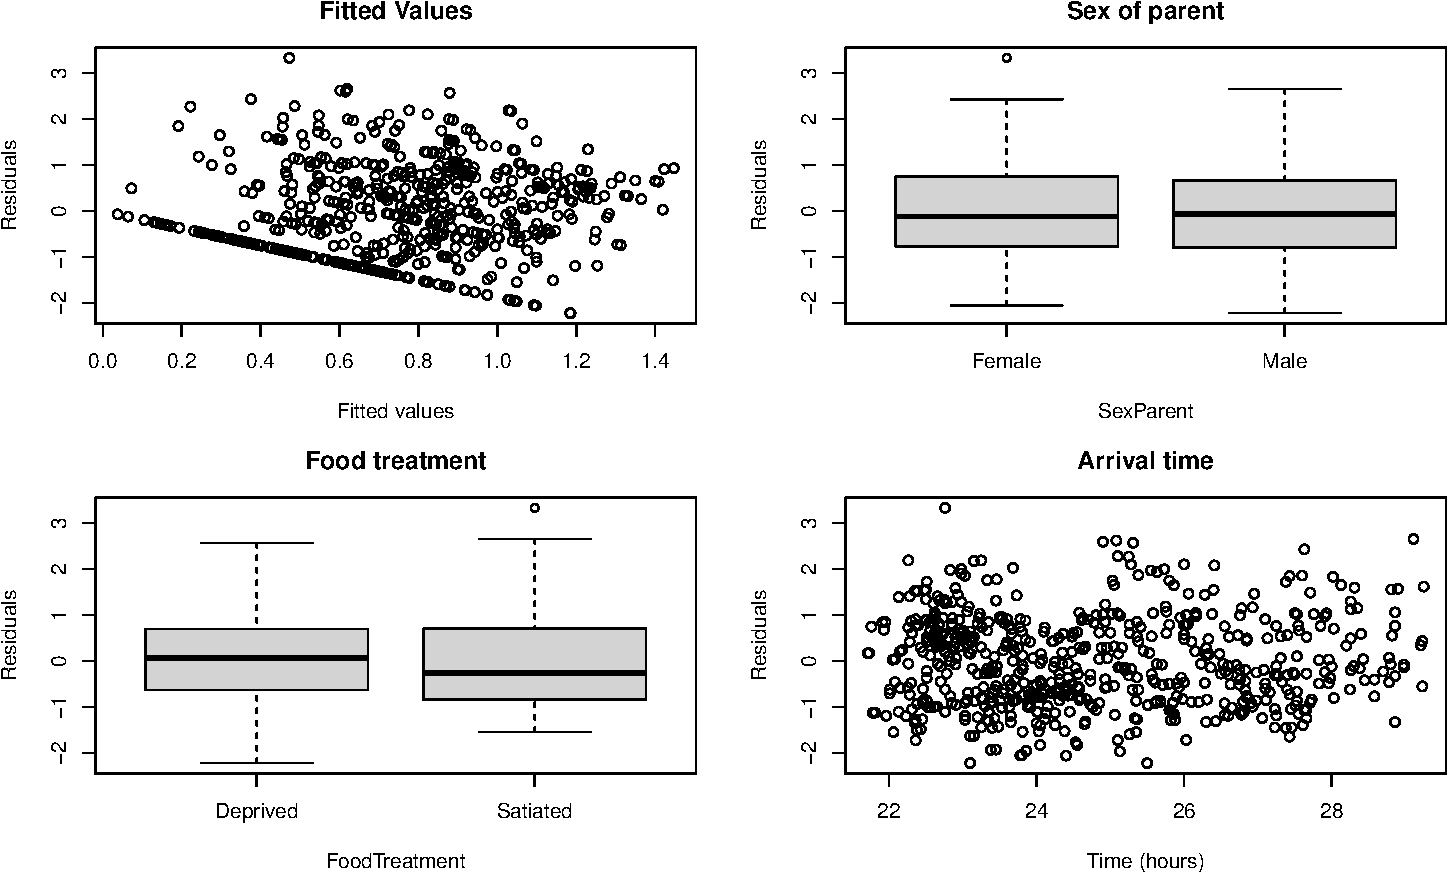
\includegraphics{mixed_models_files/figure-beamer/unnamed-chunk-16-1.pdf}
\end{frame}

\begin{frame}[fragile]{Summary of the mixed model}
\protect\hypertarget{summary-of-the-mixed-model}{}
\tiny

\begin{verbatim}
## Linear mixed-effects model fit by REML
##   Data: Owls 
##        AIC     BIC   logLik
##   1026.878 1061.96 -505.439
## 
## Random effects:
##  Formula: ~1 | Nest
##         (Intercept)  Residual
## StdDev:   0.2143996 0.5345205
## 
## Fixed effects:  list(Form) 
##                                          Value Std.Error  DF   t-value p-value
## (Intercept)                          2.5872800 0.4495127 567  5.755744  0.0000
## SexParentMale                        0.2491715 0.5861657 567  0.425087  0.6709
## FoodTreatmentSatiated               -0.4188292 0.0705245 567 -5.938776  0.0000
## ArrivalTime                         -0.0667932 0.0180023 567 -3.710251  0.0002
## SexParentMale:FoodTreatmentSatiated  0.0322772 0.0914373 567  0.352998  0.7242
## SexParentMale:ArrivalTime           -0.0088322 0.0234809 567 -0.376144  0.7070
##  Correlation: 
##                                     (Intr) SxPrnM FdTrtS ArrvlT SPM:FT
## SexParentMale                       -0.749                            
## FoodTreatmentSatiated               -0.102  0.080                     
## ArrivalTime                         -0.989  0.746  0.022              
## SexParentMale:FoodTreatmentSatiated  0.078 -0.113 -0.756 -0.019       
## SexParentMale:ArrivalTime            0.747 -0.994 -0.019 -0.755  0.037
## 
## Standardized Within-Group Residuals:
##        Min         Q1        Med         Q3        Max 
## -2.2182205 -0.7902406 -0.0778161  0.6991138  3.3273193 
## 
## Number of Observations: 599
## Number of Groups: 27
\end{verbatim}
\end{frame}

\begin{frame}[fragile]{Model selection}
\protect\hypertarget{model-selection}{}
\tiny

\begin{Shaded}
\begin{Highlighting}[]
\NormalTok{M1.lmeML}\OtherTok{=}\FunctionTok{lme}\NormalTok{(Form,}\AttributeTok{random=}\SpecialCharTok{\textasciitilde{}}\DecValTok{1}\SpecialCharTok{|}\NormalTok{Nest,}\AttributeTok{method=}\StringTok{"ML"}\NormalTok{,}\AttributeTok{data=}\NormalTok{Owls)}
\FunctionTok{dredge}\NormalTok{(M1.lmeML)}
\end{Highlighting}
\end{Shaded}

\begin{verbatim}
## Global model call: lme.formula(fixed = Form, data = Owls, random = ~1 | Nest, method = "ML")
## ---
## Model selection table 
##     (Int)      ArT FdT SxP ArT:SxP FdT:SxP df   logLik   AICc delta weight
## 4  2.7200 -0.07137   +                      5 -491.813  993.7  0.00  0.476
## 8  2.7030 -0.07191   +   +                  6 -491.347  994.8  1.11  0.273
## 16 2.5750 -0.06670   +   +       +          7 -491.273  996.7  3.01  0.106
## 24 2.7110 -0.07185   +   +               +  7 -491.280  996.8  3.02  0.105
## 32 2.5870 -0.06682   +   +       +       +  8 -491.211  998.7  4.94  0.040
## 3  0.9475            +                      4 -509.674 1027.4 33.69  0.000
## 7  0.9253            +   +                  5 -509.444 1029.0 35.26  0.000
## 23 0.9371            +   +               +  6 -509.354 1030.9 37.12  0.000
## 6  2.3950 -0.06804       +                  5 -526.370 1062.8 69.11  0.000
## 2  2.4220 -0.06712                          4 -527.605 1063.3 69.55  0.000
## 14 2.3170 -0.06488       +       +          6 -526.346 1064.8 71.11  0.000
## 1  0.7604                                   3 -541.668 1089.4 95.65  0.000
## 5  0.7189                +                  4 -540.826 1089.7 95.99  0.000
## Models ranked by AICc(x) 
## Random terms (all models): 
## '1 | Nest'
\end{verbatim}

\normalsize

Sex of the parent is not quite a significant predictor according to AIC.
It is close though. Perhaps there is more work to do.
\end{frame}

\begin{frame}[fragile]{Fit the optimal linear mixed model}
\protect\hypertarget{fit-the-optimal-linear-mixed-model}{}
Sex of the parent is not a predictor. \tiny

\begin{Shaded}
\begin{Highlighting}[]
\NormalTok{M1.opt }\OtherTok{\textless{}{-}} \FunctionTok{lme}\NormalTok{(LogNeg}\SpecialCharTok{\textasciitilde{}}\NormalTok{FoodTreatment}\SpecialCharTok{+}\NormalTok{ArrivalTime,}\AttributeTok{random=}\SpecialCharTok{\textasciitilde{}}\DecValTok{1}\SpecialCharTok{|}\NormalTok{Nest,}\AttributeTok{data=}\NormalTok{Owls)}
\FunctionTok{summary}\NormalTok{(M1.opt)}
\end{Highlighting}
\end{Shaded}

\begin{verbatim}
## Linear mixed-effects model fit by REML
##   Data: Owls 
##        AIC      BIC    logLik
##   1009.241 1031.192 -499.6203
## 
## Random effects:
##  Formula: ~1 | Nest
##         (Intercept)  Residual
## StdDev:   0.2180265 0.5333704
## 
## Fixed effects:  LogNeg ~ FoodTreatment + ArrivalTime 
##                            Value  Std.Error  DF   t-value p-value
## (Intercept)            2.7219747 0.29697570 570  9.165648       0
## FoodTreatmentSatiated -0.4031260 0.04597355 570 -8.768650       0
## ArrivalTime           -0.0714293 0.01177156 570 -6.067954       0
##  Correlation: 
##                       (Intr) FdTrtS
## FoodTreatmentSatiated -0.112       
## ArrivalTime           -0.984  0.039
## 
## Standardized Within-Group Residuals:
##         Min          Q1         Med          Q3         Max 
## -2.22283609 -0.78307304 -0.07461892  0.68690000  3.29183331 
## 
## Number of Observations: 599
## Number of Groups: 27
\end{verbatim}
\end{frame}

\begin{frame}[fragile]{What if we don't use \texttt{Nest} as a random
effect?}
\protect\hypertarget{what-if-we-dont-use-nest-as-a-random-effect}{}
\scriptsize

\begin{Shaded}
\begin{Highlighting}[]
\NormalTok{M1.wrong}\OtherTok{=}\FunctionTok{lm}\NormalTok{(LogNeg}\SpecialCharTok{\textasciitilde{}}\NormalTok{SexParent}\SpecialCharTok{*}\NormalTok{(FoodTreatment}\SpecialCharTok{+}\NormalTok{ArrivalTime)}\SpecialCharTok{+}\NormalTok{Nest,}\AttributeTok{data=}\NormalTok{Owls)}
\FunctionTok{Anova}\NormalTok{(M1.wrong)}
\end{Highlighting}
\end{Shaded}

\begin{verbatim}
## Anova Table (Type II tests)
## 
## Response: LogNeg
##                          Sum Sq  Df F value    Pr(>F)    
## SexParent                 0.106   1  0.3745    0.5408    
## FoodTreatment            22.383   1 79.0186 < 2.2e-16 ***
## ArrivalTime              10.865   1 38.3571 1.132e-09 ***
## Nest                     28.654  26  3.8907 8.526e-10 ***
## SexParent:FoodTreatment   0.049   1  0.1716    0.6789    
## SexParent:ArrivalTime     0.087   1  0.3074    0.5795    
## Residuals               160.607 567                      
## ---
## Signif. codes:  0 '***' 0.001 '**' 0.01 '*' 0.05 '.' 0.1 ' ' 1
\end{verbatim}

\normalsize

The result is similar, but it applies \emph{only} to these 27 nests.
\end{frame}

\begin{frame}[fragile]{Comparison of parameter estimates}
\protect\hypertarget{comparison-of-parameter-estimates}{}
They are almost identical. The mixed model predicts a 3-6\% smaller
effect of food treatment.

\scriptsize

\begin{Shaded}
\begin{Highlighting}[]
\FunctionTok{intervals}\NormalTok{(M1.lme)}\SpecialCharTok{$}\NormalTok{fixed[}\DecValTok{2}\SpecialCharTok{:}\DecValTok{4}\NormalTok{, }\FunctionTok{c}\NormalTok{(}\DecValTok{1}\NormalTok{,}\DecValTok{3}\NormalTok{)]}
\end{Highlighting}
\end{Shaded}

\begin{verbatim}
##                            lower       upper
## SexParentMale         -0.9021498  1.40049288
## FoodTreatmentSatiated -0.5573504 -0.28030806
## ArrivalTime           -0.1021526 -0.03143379
\end{verbatim}

\begin{Shaded}
\begin{Highlighting}[]
\FunctionTok{apply}\NormalTok{(}\FunctionTok{intervals}\NormalTok{(M1.lme)}\SpecialCharTok{$}\NormalTok{fixed[}\DecValTok{2}\SpecialCharTok{:}\DecValTok{4}\NormalTok{, }\FunctionTok{c}\NormalTok{(}\DecValTok{1}\NormalTok{,}\DecValTok{3}\NormalTok{)], }\DecValTok{1}\NormalTok{, diff)}
\end{Highlighting}
\end{Shaded}

\begin{verbatim}
##         SexParentMale FoodTreatmentSatiated           ArrivalTime 
##            2.30264266            0.27704233            0.07071885
\end{verbatim}

\begin{Shaded}
\begin{Highlighting}[]
\FunctionTok{confint}\NormalTok{(M1.wrong)[}\DecValTok{2}\SpecialCharTok{:}\DecValTok{4}\NormalTok{,]}
\end{Highlighting}
\end{Shaded}

\begin{verbatim}
##                            2.5 %     97.5 %
## SexParentMale         -0.8178743  1.4865913
## FoodTreatmentSatiated -0.5772142 -0.2988176
## ArrivalTime           -0.1015671 -0.0308154
\end{verbatim}

\begin{Shaded}
\begin{Highlighting}[]
\FunctionTok{apply}\NormalTok{(}\FunctionTok{confint}\NormalTok{(M1.wrong)[}\DecValTok{2}\SpecialCharTok{:}\DecValTok{4}\NormalTok{,], }\DecValTok{1}\NormalTok{, diff)}
\end{Highlighting}
\end{Shaded}

\begin{verbatim}
##         SexParentMale FoodTreatmentSatiated           ArrivalTime 
##            2.30446563            0.27839658            0.07075168
\end{verbatim}
\end{frame}

\begin{frame}[fragile]{Comparison of predictions}
\protect\hypertarget{comparison-of-predictions}{}
The model where \texttt{Nest} is a random effect makes predictions that
are closer to the overall mean.

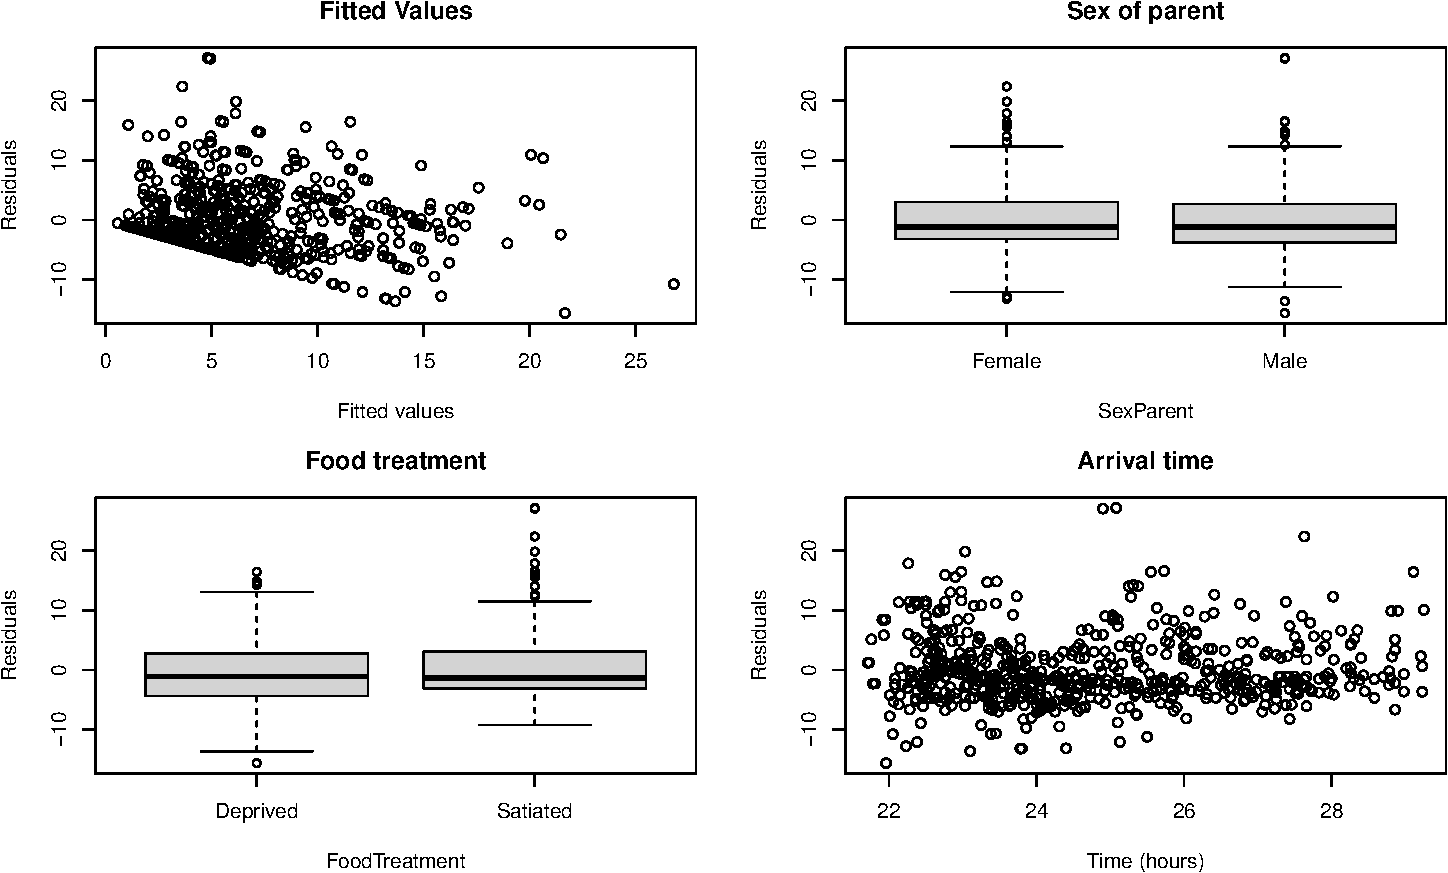
\includegraphics{mixed_models_files/figure-beamer/unnamed-chunk-22-1.pdf}
\end{frame}

\begin{frame}[fragile]{A model built with \texttt{glmmTMB}}
\protect\hypertarget{a-model-built-with-glmmtmb}{}
Instead of log-transforming the negotiations, we could use a log link
and a negative binomial error distribution.

\begin{itemize}
\tightlist
\item
  Include \texttt{offset(BroodSize)} instead of using
  \texttt{NegPerChick}.
\item
  Random effect of \texttt{1\textbar{}Nest} is included in the main
  formula.
\item
  Include zero inflation with \texttt{zi\ =\ \textasciitilde{}1}. The
  formula \texttt{\textasciitilde{}1} means that we expect there to be
  excess zeros in the data but we do not propose a reason for them.
\end{itemize}

\scriptsize

\begin{Shaded}
\begin{Highlighting}[]
\NormalTok{M.tmb}\OtherTok{\textless{}{-}}\FunctionTok{glmmTMB}\NormalTok{(SiblingNegotiation}\SpecialCharTok{\textasciitilde{}}\NormalTok{SexParent}\SpecialCharTok{*}\NormalTok{(FoodTreatment}\SpecialCharTok{+}\NormalTok{ArrivalTime)}\SpecialCharTok{+} 
\NormalTok{                    (}\DecValTok{1}\SpecialCharTok{|}\NormalTok{Nest) }\SpecialCharTok{+} \FunctionTok{offset}\NormalTok{(BroodSize),}
                    \AttributeTok{family =} \FunctionTok{nbinom1}\NormalTok{(), }\AttributeTok{zi =} \SpecialCharTok{\textasciitilde{}}\DecValTok{1}\NormalTok{, }\AttributeTok{data =}\NormalTok{ Owls)}
\end{Highlighting}
\end{Shaded}
\end{frame}

\begin{frame}{Diagnostic plots of the TMB model}
\protect\hypertarget{diagnostic-plots-of-the-tmb-model}{}
\scriptsize

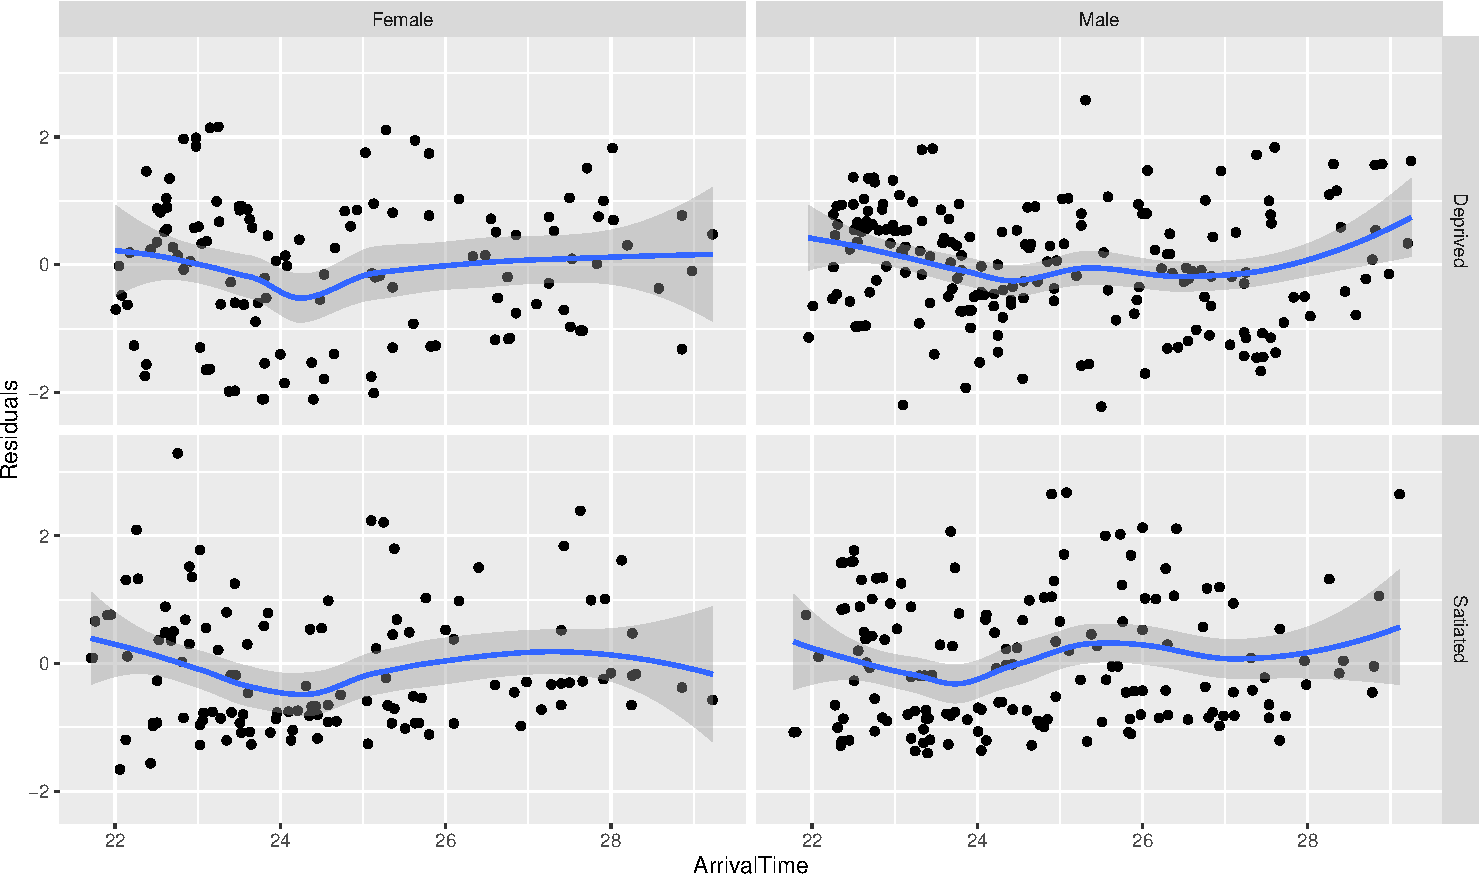
\includegraphics{mixed_models_files/figure-beamer/unnamed-chunk-24-1.pdf}
\end{frame}

\begin{frame}[fragile]{Summary of \texttt{M1.tmb}}
\protect\hypertarget{summary-of-m1.tmb}{}
\tiny

\begin{verbatim}
##  Family: nbinom1  ( log )
## Formula:          
## SiblingNegotiation ~ SexParent * (FoodTreatment + ArrivalTime) +  
##     (1 | Nest) + offset(BroodSize)
## Zero inflation:                      ~1
## Data: Owls
## 
##      AIC      BIC   logLik deviance df.resid 
##   3394.1   3433.6  -1688.0   3376.1      590 
## 
## Random effects:
## 
## Conditional model:
##  Groups Name        Variance Std.Dev.
##  Nest   (Intercept) 1.157    1.076   
## Number of obs: 599, groups:  Nest, 27
## 
## Overdispersion parameter for nbinom1 family (): 5.01 
## 
## Conditional model:
##                                     Estimate Std. Error z value Pr(>|z|)    
## (Intercept)                          0.86649    0.85366   1.015 0.310092    
## SexParentMale                        0.57261    1.04563   0.548 0.583950    
## FoodTreatmentSatiated               -0.94619    0.13788  -6.862 6.77e-12 ***
## ArrivalTime                         -0.11557    0.03400  -3.399 0.000676 ***
## SexParentMale:FoodTreatmentSatiated  0.28153    0.17318   1.626 0.104017    
## SexParentMale:ArrivalTime           -0.02681    0.04294  -0.624 0.532409    
## ---
## Signif. codes:  0 '***' 0.001 '**' 0.01 '*' 0.05 '.' 0.1 ' ' 1
## 
## Zero-inflation model:
##             Estimate Std. Error z value Pr(>|z|)    
## (Intercept)  -2.5605     0.3625  -7.063 1.63e-12 ***
## ---
## Signif. codes:  0 '***' 0.001 '**' 0.01 '*' 0.05 '.' 0.1 ' ' 1
\end{verbatim}
\end{frame}

\begin{frame}[fragile]{The effect of arrival time is not linear}
\protect\hypertarget{the-effect-of-arrival-time-is-not-linear}{}
\texttt{SexParent}-\texttt{FoodTreatment} combinations show residual
patterns.

\scriptsize

\begin{Shaded}
\begin{Highlighting}[]
\NormalTok{Owls}\SpecialCharTok{$}\NormalTok{Eopt }\OtherTok{\textless{}{-}} \FunctionTok{resid}\NormalTok{(M1.opt,}\AttributeTok{type=}\StringTok{"normalized"}\NormalTok{)}
\FunctionTok{ggplot}\NormalTok{(Owls, }\FunctionTok{aes}\NormalTok{(ArrivalTime, Eopt))}\SpecialCharTok{+} \FunctionTok{geom\_point}\NormalTok{()}\SpecialCharTok{+}\FunctionTok{geom\_smooth}\NormalTok{()}\SpecialCharTok{+}
  \FunctionTok{facet\_grid}\NormalTok{(FoodTreatment}\SpecialCharTok{\textasciitilde{}}\NormalTok{SexParent)}\SpecialCharTok{+}\FunctionTok{ylab}\NormalTok{(}\StringTok{"Residuals"}\NormalTok{)}
\end{Highlighting}
\end{Shaded}

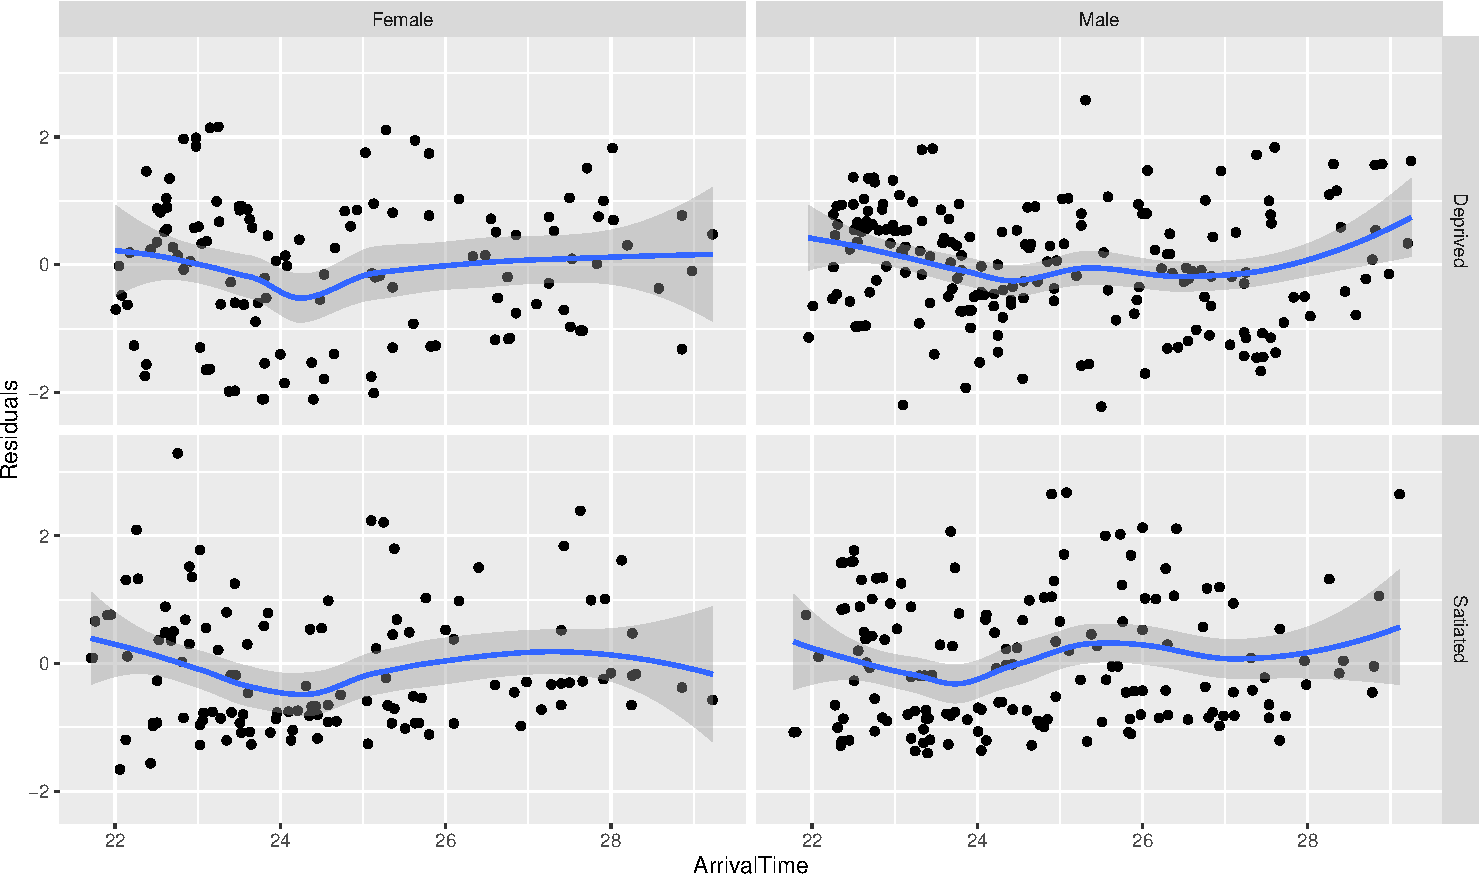
\includegraphics{mixed_models_files/figure-beamer/unnamed-chunk-26-1.pdf}
\end{frame}

\begin{frame}[fragile]{GAMM}
\protect\hypertarget{gamm}{}
A generalized additive mixed model gives flexibility to include
nonlinear effects.

\begin{itemize}
\tightlist
\item
  A black-box smooth function relating \texttt{ArrivalTime} to
  \texttt{SiblingNegotiation} is created with \texttt{s()}.
\item
  Including \texttt{by=SexParent} substitutes for the interaction.
\item
  Random effects go in a \texttt{list}.
\item
  Negative binomial errors aren't an option so we use Poisson.
\end{itemize}

\scriptsize

\begin{Shaded}
\begin{Highlighting}[]
\NormalTok{M.gamm}\OtherTok{\textless{}{-}}\FunctionTok{gamm}\NormalTok{(SiblingNegotiation}\SpecialCharTok{\textasciitilde{}}\FunctionTok{offset}\NormalTok{(BroodSize)}\SpecialCharTok{+}
\NormalTok{                SexParent}\SpecialCharTok{*}\NormalTok{FoodTreatment}\SpecialCharTok{+}\FunctionTok{s}\NormalTok{(ArrivalTime, }\AttributeTok{by=}\NormalTok{SexParent),}
              \AttributeTok{random=}\FunctionTok{list}\NormalTok{(}\AttributeTok{Nest=}\SpecialCharTok{\textasciitilde{}}\DecValTok{1}\NormalTok{),}\AttributeTok{data=}\NormalTok{Owls,}
              \AttributeTok{family=}\NormalTok{poisson)}
\end{Highlighting}
\end{Shaded}

\begin{verbatim}
## 
##  Maximum number of PQL iterations:  20
\end{verbatim}
\end{frame}

\begin{frame}{Diagnostic plots of the generalized additive mixed model}
\protect\hypertarget{diagnostic-plots-of-the-generalized-additive-mixed-model}{}
\scriptsize

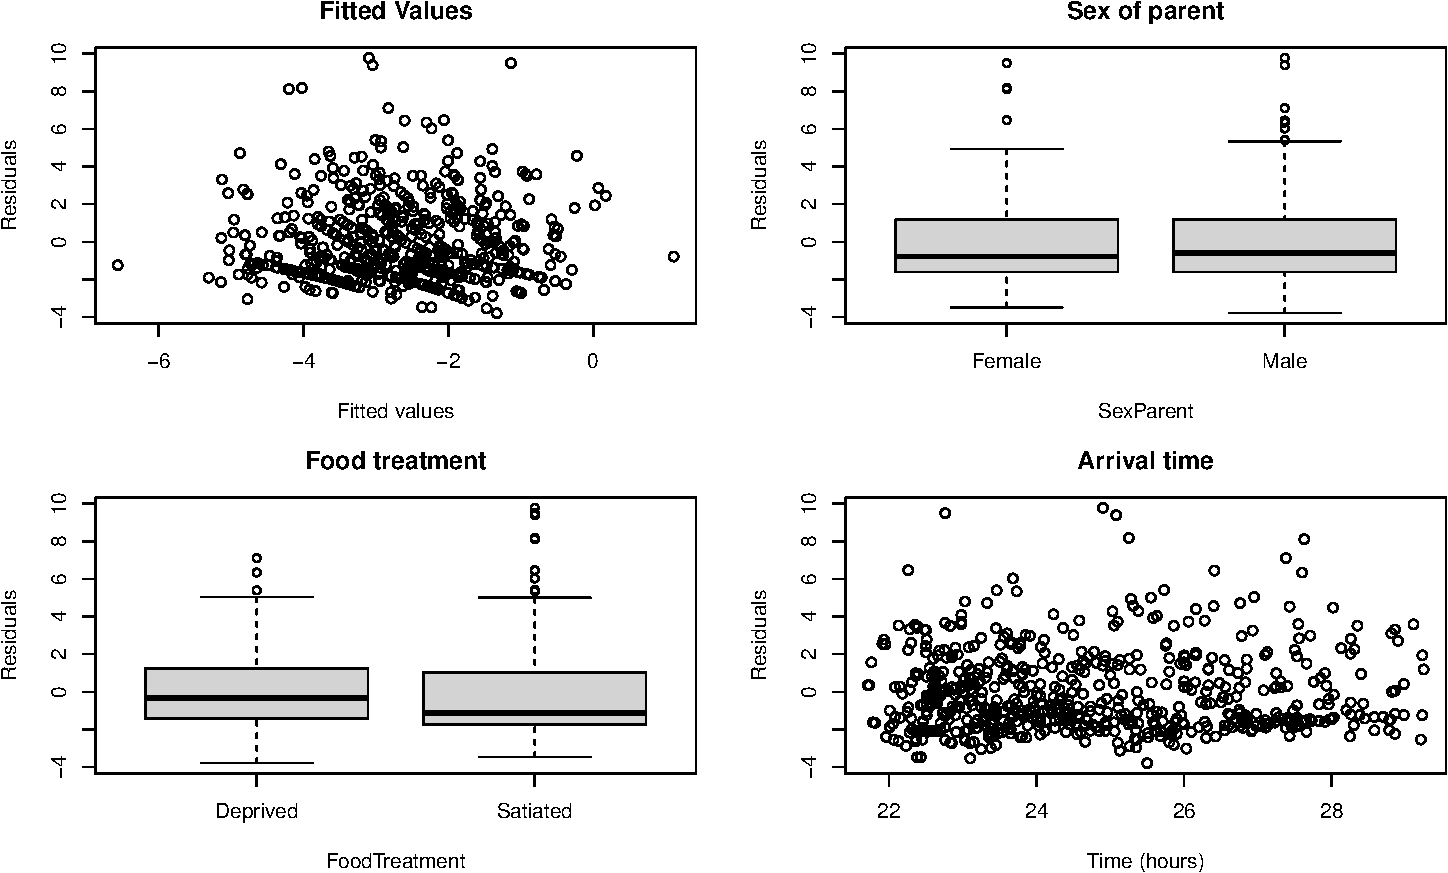
\includegraphics{mixed_models_files/figure-beamer/unnamed-chunk-28-1.pdf}
\end{frame}

\begin{frame}[fragile]{Using a GAMM straightens out the residuals}
\protect\hypertarget{using-a-gamm-straightens-out-the-residuals}{}
\scriptsize

\begin{Shaded}
\begin{Highlighting}[]
\NormalTok{Owls}\SpecialCharTok{$}\NormalTok{Egamm }\OtherTok{\textless{}{-}} \FunctionTok{resid}\NormalTok{(M.gamm,}\AttributeTok{type=}\StringTok{"normalized"}\NormalTok{)}
\FunctionTok{ggplot}\NormalTok{(Owls, }\FunctionTok{aes}\NormalTok{(ArrivalTime, Egamm))}\SpecialCharTok{+} \FunctionTok{geom\_point}\NormalTok{()}\SpecialCharTok{+}\FunctionTok{geom\_smooth}\NormalTok{()}\SpecialCharTok{+}
  \FunctionTok{facet\_grid}\NormalTok{(FoodTreatment}\SpecialCharTok{\textasciitilde{}}\NormalTok{SexParent)}\SpecialCharTok{+}\FunctionTok{ylab}\NormalTok{(}\StringTok{"Residuals"}\NormalTok{)}
\end{Highlighting}
\end{Shaded}

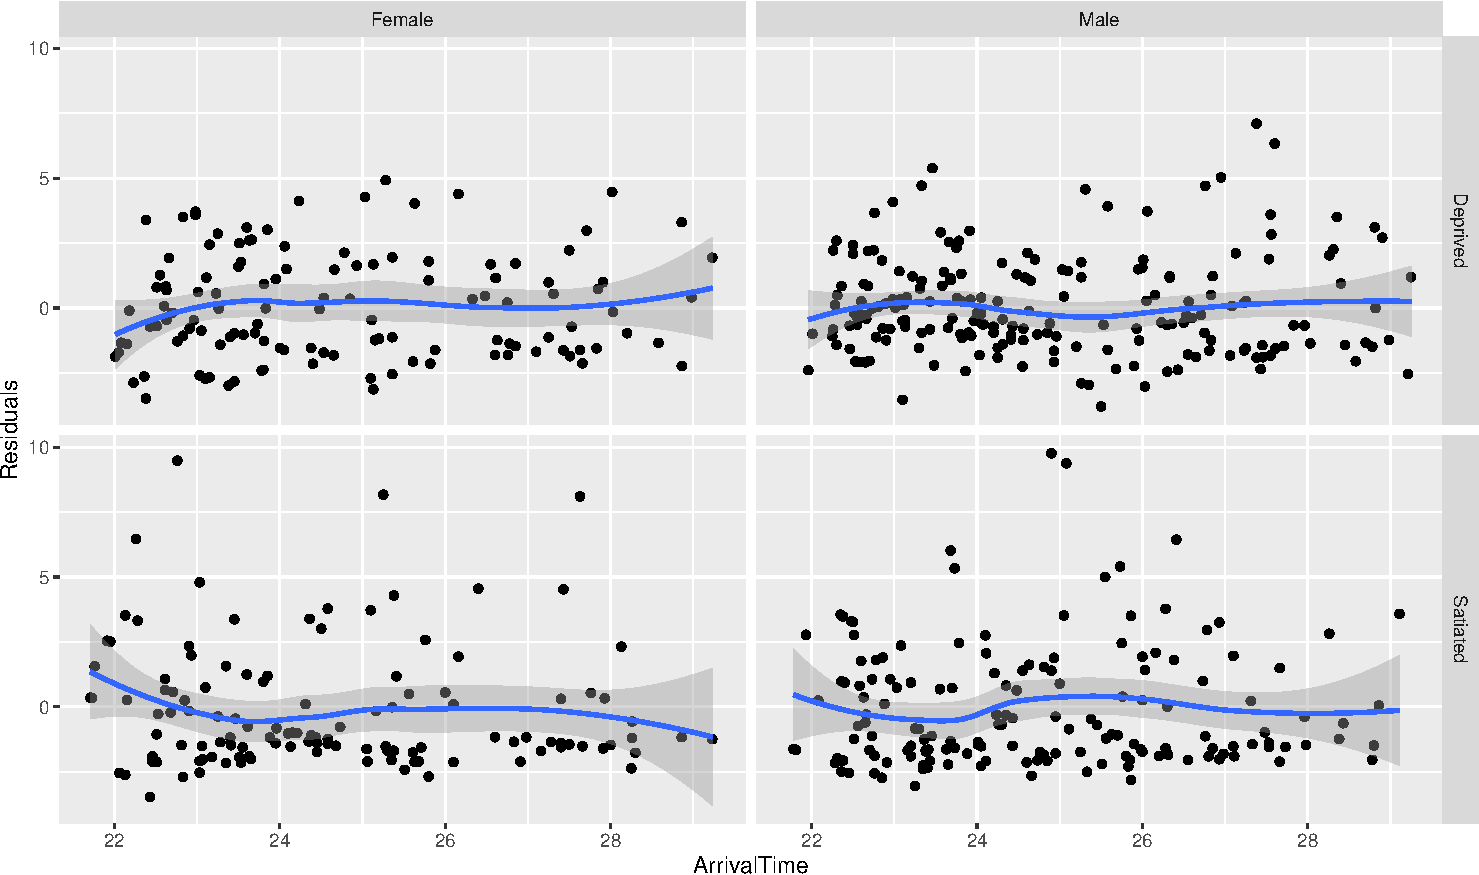
\includegraphics{mixed_models_files/figure-beamer/unnamed-chunk-29-1.pdf}
\end{frame}

\begin{frame}[fragile]{Summary of \texttt{M.gamm\$gam}}
\protect\hypertarget{summary-of-m.gammgam}{}
\tiny

\begin{verbatim}
## 
## Family: poisson 
## Link function: log 
## 
## Formula:
## SiblingNegotiation ~ offset(BroodSize) + SexParent * FoodTreatment + 
##     s(ArrivalTime, by = SexParent)
## 
## Parametric coefficients:
##                                     Estimate Std. Error t value Pr(>|t|)    
## (Intercept)                         -2.17039    0.23417  -9.268   <2e-16 ***
## SexParentMale                       -0.00743    0.04830  -0.154   0.8778    
## FoodTreatmentSatiated               -0.68125    0.05721 -11.908   <2e-16 ***
## SexParentMale:FoodTreatmentSatiated  0.14333    0.07172   1.998   0.0461 *  
## ---
## Signif. codes:  0 '***' 0.001 '**' 0.01 '*' 0.05 '.' 0.1 ' ' 1
## 
## Approximate significance of smooth terms:
##                                  edf Ref.df     F p-value    
## s(ArrivalTime):SexParentFemale 8.324  8.324 24.82  <2e-16 ***
## s(ArrivalTime):SexParentMale   8.096  8.096 35.85  <2e-16 ***
## ---
## Signif. codes:  0 '***' 0.001 '**' 0.01 '*' 0.05 '.' 0.1 ' ' 1
## 
## R-sq.(adj) =  -16.2   
##   Scale est. = 1         n = 599
\end{verbatim}

Baby Owl says, ``Hey Papa, bring us another mouse! The one the
scientists left for us smells funny.''
\end{frame}

\begin{frame}[fragile]{F tests on the GAMM}
\protect\hypertarget{f-tests-on-the-gamm}{}
\scriptsize

\begin{Shaded}
\begin{Highlighting}[]
\FunctionTok{anova}\NormalTok{(M.gamm}\SpecialCharTok{$}\NormalTok{gam)}
\end{Highlighting}
\end{Shaded}

\begin{verbatim}
## 
## Family: poisson 
## Link function: log 
## 
## Formula:
## SiblingNegotiation ~ offset(BroodSize) + SexParent * FoodTreatment + 
##     s(ArrivalTime, by = SexParent)
## 
## Parametric Terms:
##                         df       F p-value
## SexParent                1   0.024  0.8778
## FoodTreatment            1 141.794  <2e-16
## SexParent:FoodTreatment  1   3.994  0.0461
## 
## Approximate significance of smooth terms:
##                                  edf Ref.df     F p-value
## s(ArrivalTime):SexParentFemale 8.324  8.324 24.82  <2e-16
## s(ArrivalTime):SexParentMale   8.096  8.096 35.85  <2e-16
\end{verbatim}
\end{frame}

\begin{frame}[fragile]{Summary of \texttt{M.gamm\$lme}}
\protect\hypertarget{summary-of-m.gammlme}{}
\texttt{summary(M.gamm\$lme)} includes the correlation matrix.

\begin{itemize}
\tightlist
\item
  Highly correlated parameters may warrant an explanation.
\item
  Intercept is often highly correlated with slope for variables in
  linear models that are not centered.
\item
  Interaction terms tend to be correlated with the interacting
  variables.
\end{itemize}

\scriptsize

\begin{Shaded}
\begin{Highlighting}[]
\NormalTok{sml }\OtherTok{\textless{}{-}} \FunctionTok{summary}\NormalTok{(M.gamm}\SpecialCharTok{$}\NormalTok{lme)}
\FunctionTok{colnames}\NormalTok{(sml}\SpecialCharTok{$}\NormalTok{corFixed) }\OtherTok{\textless{}{-}} \FunctionTok{abbreviate}\NormalTok{(}\FunctionTok{colnames}\NormalTok{(sml}\SpecialCharTok{$}\NormalTok{corFixed), }\AttributeTok{minlength=}\DecValTok{8}\NormalTok{)}
\FunctionTok{rownames}\NormalTok{(sml}\SpecialCharTok{$}\NormalTok{corFixed) }\OtherTok{\textless{}{-}} \FunctionTok{abbreviate}\NormalTok{(}\FunctionTok{rownames}\NormalTok{(sml}\SpecialCharTok{$}\NormalTok{corFixed), }\AttributeTok{minlength=}\DecValTok{8}\NormalTok{)}
\FunctionTok{round}\NormalTok{(sml}\SpecialCharTok{$}\NormalTok{corFixed,}\DecValTok{3}\NormalTok{)}
\end{Highlighting}
\end{Shaded}

\begin{verbatim}
##           X(Intrc) XSxPrntM XFdTrtmS XSPM:FTS X(AT):SPF X(AT):SPM
## X(Intrc)     1.000   -0.130   -0.092    0.069     0.007     0.001
## XSxPrntM    -0.130    1.000    0.457   -0.569    -0.043    -0.090
## XFdTrtmS    -0.092    0.457    1.000   -0.769     0.093    -0.001
## XSPM:FTS     0.069   -0.569   -0.769    1.000    -0.067     0.034
## X(AT):SPF    0.007   -0.043    0.093   -0.067     1.000     0.003
## X(AT):SPM    0.001   -0.090   -0.001    0.034     0.003     1.000
\end{verbatim}
\end{frame}

\begin{frame}[fragile]{AIC and significance of \texttt{SexParent}}
\protect\hypertarget{aic-and-significance-of-sexparent}{}
Fitting a model without \texttt{SexParent} gives a much higher AIC.

\scriptsize

\begin{Shaded}
\begin{Highlighting}[]
\NormalTok{M2.gamm }\OtherTok{\textless{}{-}} \FunctionTok{gamm}\NormalTok{(SiblingNegotiation}\SpecialCharTok{\textasciitilde{}}\FunctionTok{offset}\NormalTok{(BroodSize)}\SpecialCharTok{+}
\NormalTok{                SexParent}\SpecialCharTok{+}\NormalTok{FoodTreatment}\SpecialCharTok{+}\FunctionTok{s}\NormalTok{(ArrivalTime, }\AttributeTok{by=}\NormalTok{SexParent),}
                \AttributeTok{random=}\FunctionTok{list}\NormalTok{(}\AttributeTok{Nest=}\SpecialCharTok{\textasciitilde{}}\DecValTok{1}\NormalTok{), }\AttributeTok{data=}\NormalTok{Owls, }\AttributeTok{family=}\NormalTok{poisson)}
\NormalTok{M3.gamm }\OtherTok{\textless{}{-}} \FunctionTok{gamm}\NormalTok{(SiblingNegotiation}\SpecialCharTok{\textasciitilde{}}\FunctionTok{offset}\NormalTok{(BroodSize)}\SpecialCharTok{+}
\NormalTok{                SexParent}\SpecialCharTok{*}\NormalTok{FoodTreatment}\SpecialCharTok{+}\FunctionTok{s}\NormalTok{(ArrivalTime),}
                \AttributeTok{random=}\FunctionTok{list}\NormalTok{(}\AttributeTok{Nest=}\SpecialCharTok{\textasciitilde{}}\DecValTok{1}\NormalTok{), }\AttributeTok{data=}\NormalTok{Owls, }\AttributeTok{family=}\NormalTok{poisson)}
\NormalTok{M4.gamm }\OtherTok{\textless{}{-}} \FunctionTok{gamm}\NormalTok{(SiblingNegotiation}\SpecialCharTok{\textasciitilde{}}\FunctionTok{offset}\NormalTok{(BroodSize)}\SpecialCharTok{+}
\NormalTok{                SexParent}\SpecialCharTok{+}\NormalTok{FoodTreatment}\SpecialCharTok{+}\FunctionTok{s}\NormalTok{(ArrivalTime),}
                \AttributeTok{random=}\FunctionTok{list}\NormalTok{(}\AttributeTok{Nest=}\SpecialCharTok{\textasciitilde{}}\DecValTok{1}\NormalTok{), }\AttributeTok{data=}\NormalTok{Owls, }\AttributeTok{family=}\NormalTok{poisson)}
\NormalTok{M5.gamm }\OtherTok{\textless{}{-}} \FunctionTok{gamm}\NormalTok{(SiblingNegotiation}\SpecialCharTok{\textasciitilde{}}\FunctionTok{offset}\NormalTok{(BroodSize)}\SpecialCharTok{+}
\NormalTok{                FoodTreatment}\SpecialCharTok{+}\FunctionTok{s}\NormalTok{(ArrivalTime),}
                \AttributeTok{random=}\FunctionTok{list}\NormalTok{(}\AttributeTok{Nest=}\SpecialCharTok{\textasciitilde{}}\DecValTok{1}\NormalTok{), }\AttributeTok{data=}\NormalTok{Owls, }\AttributeTok{family=}\NormalTok{poisson)}
\end{Highlighting}
\end{Shaded}

\scriptsize

\begin{Shaded}
\begin{Highlighting}[]
\FunctionTok{AIC}\NormalTok{(M.gamm, M2.gamm, M3.gamm, M4.gamm, M5.gamm)}
\end{Highlighting}
\end{Shaded}

\begin{verbatim}
##         df      AIC
## M.gamm   9 3107.012
## M2.gamm  8 3105.906
## M3.gamm  7 3179.468
## M4.gamm  6 3179.027
## M5.gamm  5 3177.889
\end{verbatim}
\end{frame}

\begin{frame}[fragile]{Summary of \texttt{M2.gamm\$gam}}
\protect\hypertarget{summary-of-m2.gammgam}{}
\tiny

\begin{verbatim}
## 
## Family: poisson 
## Link function: log 
## 
## Formula:
## SiblingNegotiation ~ offset(BroodSize) + SexParent + FoodTreatment + 
##     s(ArrivalTime, by = SexParent)
## 
## Parametric coefficients:
##                       Estimate Std. Error t value Pr(>|t|)    
## (Intercept)           -2.20314    0.23392  -9.418   <2e-16 ***
## SexParentMale          0.04768    0.03977   1.199    0.231    
## FoodTreatmentSatiated -0.59379    0.03659 -16.230   <2e-16 ***
## ---
## Signif. codes:  0 '***' 0.001 '**' 0.01 '*' 0.05 '.' 0.1 ' ' 1
## 
## Approximate significance of smooth terms:
##                                  edf Ref.df     F p-value    
## s(ArrivalTime):SexParentFemale 8.309  8.309 24.93  <2e-16 ***
## s(ArrivalTime):SexParentMale   8.093  8.093 35.91  <2e-16 ***
## ---
## Signif. codes:  0 '***' 0.001 '**' 0.01 '*' 0.05 '.' 0.1 ' ' 1
## 
## R-sq.(adj) =  -16.5   
##   Scale est. = 1         n = 599
\end{verbatim}

Or, maybe Papa Owl and Mama Owl just visit at different times.
\end{frame}

\begin{frame}[fragile]{The smooth approximators}
\protect\hypertarget{the-smooth-approximators}{}
\begin{Shaded}
\begin{Highlighting}[]
\FunctionTok{plot}\NormalTok{(M.gamm}\SpecialCharTok{$}\NormalTok{gam)}
\end{Highlighting}
\end{Shaded}

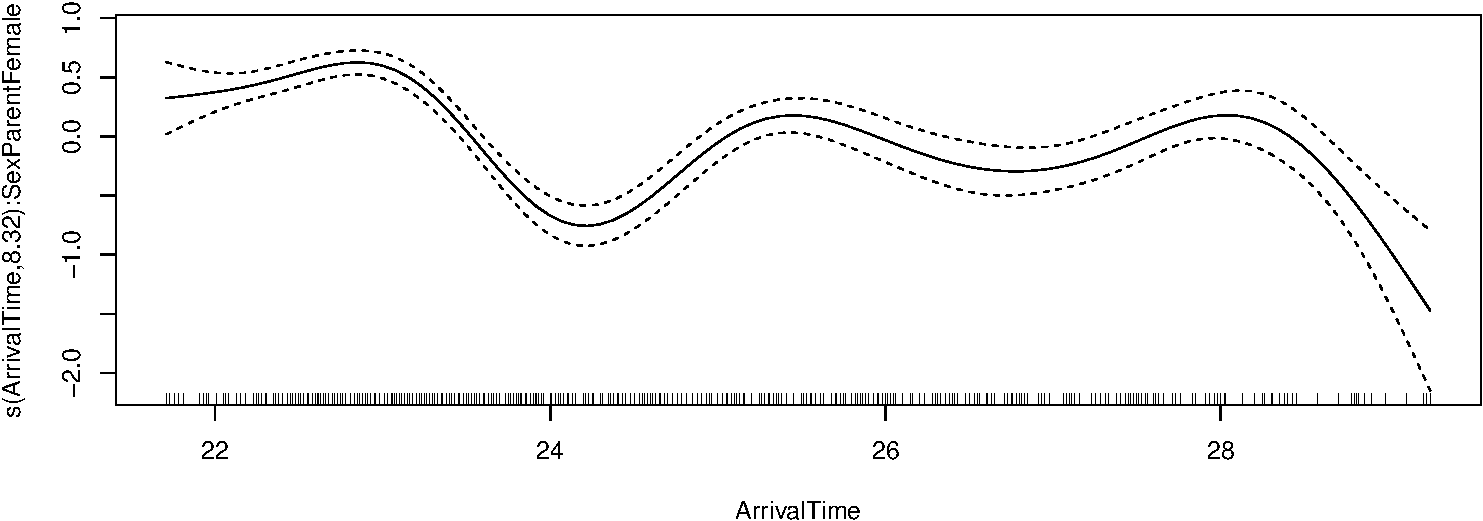
\includegraphics{mixed_models_files/figure-beamer/unnamed-chunk-36-1.pdf}
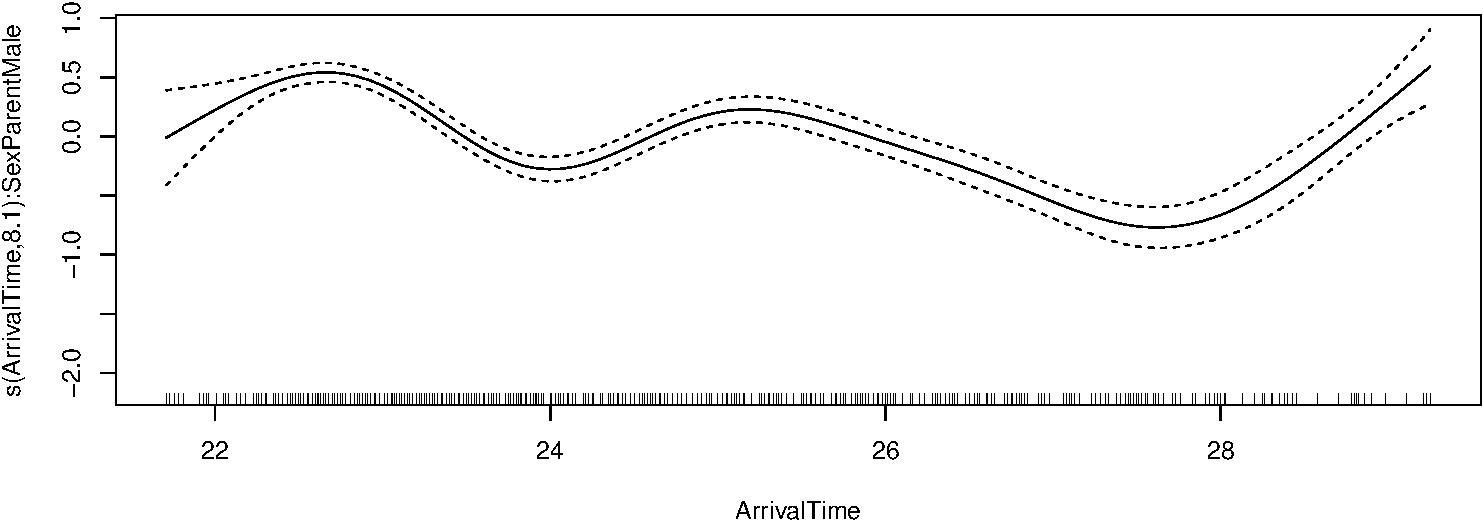
\includegraphics{mixed_models_files/figure-beamer/unnamed-chunk-36-2.pdf}
\end{frame}

\begin{frame}[fragile]{Questioning the result}
\protect\hypertarget{questioning-the-result}{}
The p-value for \texttt{SexParent:FoodTreatmentSatiated} is just barely
significant at the \(\alpha=0.05\) level, and removing it gives a small
improvement in AIC, so we should definitely temper our enthusiasm.

\begin{itemize}
\tightlist
\item
  Are we overfitting?
\item
  Is the effect size large enough to care about?
\end{itemize}

Cross validation and simulation could help answer these questions.
\end{frame}

\begin{frame}[fragile]{Enough owl models already}
\protect\hypertarget{enough-owl-models-already}{}
Roulin and Bersier (2007) finds that the sex of the parent \emph{is}
significant without going further than a linear mixed model.

The analysis there seems to hinge on the variable \emph{amount of time
in nestbox} which is missing from the data provided in Zuur et al.
(2009) (which is the source of the data in \texttt{glmmTMB::Owls}).
\end{frame}

\begin{frame}{Mixed model formula cheatsheet}
\protect\hypertarget{mixed-model-formula-cheatsheet}{}
\(Y\) is the response variable, \(X\) is a fixed effect variable, \(S\)
and \(T\) are random effect variables. Random terms \(b\) are normally
distributed with parameters determined by the variables in the
subscript.

\scriptsize
\begin{tabular}{p{3.5cm}|p{3.5cm}|p{3.5cm}}
Modeling goal & Formula specification & Mathematical specification $Y\sim$ \\
\hline
fixed effect only model & NA & $\beta_0 + \beta_1X + \epsilon$\\
random group intercept & \texttt{(1|group)} & $(\beta_0 + b_{0S}) + \beta_1X + \epsilon$\\
random slope of $X$ within group with correlated intercept & \texttt{(x|group) = (1+x|group)} 
& $(\beta_0 + b_{0S}) +  (\beta_1 + b_{1S}) X + \epsilon$\\
random slope of $X$ within group, no variation in intercept & \texttt{(0+x|group) = (-1+x|group)} 
& $\beta_0  +  (\beta_1 + b_{1S}) X + \epsilon$\\
intercept varying among sites and among blocks within sites (nested random effects) 
& \texttt{(1|site/block) = (1|site)+(1|site:block)} 
&  $(\beta_0 + b_{0S} + b_{0ST}) + \beta_1X + \epsilon$\\
intercept varying among crossed random effects (e.g. site, year) 
& \texttt{(1|group1)+(1|group2)} & $(\beta_0 + b_{0S} + b_{0T}) + \beta_1X + \epsilon$

\end{tabular}
\end{frame}

\begin{frame}{References}
\protect\hypertarget{references}{}
\hypertarget{refs}{}
\begin{CSLReferences}{1}{0}
\leavevmode\vadjust pre{\hypertarget{ref-owls}{}}%
Roulin, Alexandre, and Louis-Felix Bersier. 2007. {``Nestling Barn Owls
Beg More Intensely in the Presence of Their Mother Than in the Presence
of Their Father.''} \emph{Animal Behaviour} 74 (4): 1099--1106.
https://doi.org/\url{https://doi.org/10.1016/j.anbehav.2007.01.027}.

\leavevmode\vadjust pre{\hypertarget{ref-zuur2009mixed}{}}%
Zuur, A., E. N. Ieno, N. Walker, A. A. Saveliev, and G. M. Smith. 2009.
\emph{Mixed Effects Models and Extensions in Ecology with r}. Statistics
for Biology and Health. Springer New York.
\url{https://books.google.com/books?id=vQUNprFZKHsC}.

\end{CSLReferences}
\end{frame}

\end{document}
